\chapter{Biologische Grundlagen}
\label{sec:bio}
\marginpar{Jens}
In diesem Kapitel sollen die für unsere Projektgruppe relevanten biologischen Grundlagen erläutert werden. Die Informationen wurden (wenn nicht anders angegeben) dem Buch \textit{Molekulare Genetik} von Rolf \citet{Knippers2006} entnommen. Dieses Kapitel behandelt dabei die folgenden Themen:
Zunächst werden wir uns (in Abschnitt \ref{sec:bio:dna}) den Aufbau der DNA (dem Träger der Erbinformation) ansehen. Anschließend wird erklärt, was Chromosomen sind (Abschnitt \ref{sec:bio:chromo}) und wie sich Pro- und Eukaryoten unterscheiden (Abschnitt \ref{sec:bio:proeukaryoten}). In Abschnitt \ref{sec:bio:zell} geht es darum, wie die DNA bei der Zellteilung verdoppelt und auf die beiden Tochterzellen aufgeteilt wird. Wir kommen anschließend (in Abschnitt \ref{sec:bio:pbsyn}) zur Protein-Biosynthese, also dem Vorgang, bei dem die auf der DNA gespeicherte Information in Proteine übersetzt wird. Abschnitt \ref{sec:bio:erb} behandelt die Vererbung und soll einige Grundbegriffe der Vererbungslehre erklären. Für unsere Projektgruppe sind vor allem Mutationen des Genoms bzw. der DNA interessant. Welche Arten von Mutationen es gibt, wird in Abschnitt \ref{sec:bio:muta} näher erläutert. Das Ende dieses Kapitels befasst sich mit den verschiedenen Methoden die Basen-Sequenz eines gegebenen DNA-Stücks zu bestimmen.  

\section{DNA}
\label{sec:bio:dna}
\marginpar{Jens}
Die Desoxyribonukleinsäure, kurz DNA\footnote{Die deutsche Abkürzung DNS wird nur noch sehr selten verwendet und ist laut Duden veraltet.} (engl. desoxyribonucleic acid), kommt in allen Lebewesen vor (d.h. zum Beispiel auch  Bakterien) und ist der Träger der Erbinformation. Die DNA enthält somit die Informationen, die die Nachkommen von ihren  Eltern geerbt haben und die für den Bau von Proteinen benötigt werden. Proteine können die verschiedensten Aufgaben  in unserem Körper übernehmen. In Abschnitt \ref{sec:bio:pbsyn:proteine} werden wir genaueres über Proteine erfahren.

DNA-Moleküle bestehen aus einen Doppelstrang von \emph{Nukleotiden}, die miteinander verbunden sind. Diese Nukleotide setzen sich wiederum aus  drei Bausteinen zusammen: Einem Zucker-Molekül (der Desoxyribose), das mit einem Phosphatrest sowie einer von vier möglichen Nukleobasen chemisch verbunden ist. Die Nukleotide können zu einem Strang zusammengesetzt werden, indem das Zuckermolekül des einen Nukleotids mit dem Phosphatrest des nächsten verbunden wird. Die  Zucker-Phosphat-Ketten eines DNA-Moleküls befinden sich im äußeren Bereich des Doppelstrangs und bilden somit das Rückgrat der DNA. Zwischen den beiden Zucker-Phosphat-Ketten sind jeweils zwei Nukleobasen über Wasserstoffbrückenbindungen miteinander verbunden\footnote{Streng genommen besteht ein DNA-Doppelstrang somit aus zwei Molekülen, da nur zwischen Zucker und Phosphatrest sowie zwischen Zucker und Nukleobase chemische Bindungen vorliegen, nicht aber zwischen den Nukleobasen.}.  

\begin{figure}[htbp]
\begin{center}
\begin{minipage}[h]{0.3\textwidth}
\begin{tabular}{rl}
Desoxyribose & \includegraphicstotab[height=12pt]{bilder/DNA_Schema_Desoxyribose} \\
Phosphatrest & \includegraphicstotab[height=12pt]{bilder/DNA_Schema_Phosphatrest} \\
Adenin (\textbf{A})& \includegraphicstotab[height=12pt]{bilder/DNA_Schema_Adenin} \\
Cytosin (\textbf{C}) & \includegraphicstotab[height=12pt]{bilder/DNA_Schema_Cytosin} \\
Guanin (\textbf{G}) & \includegraphicstotab[height=12pt]{bilder/DNA_Schema_Guanin} \\
Thymin (\textbf{T}) & \includegraphicstotab[height=12pt]{bilder/DNA_Schema_Thymin} \\
\end{tabular}
\end{minipage}
\begin{minipage}[h]{0.3\textwidth}
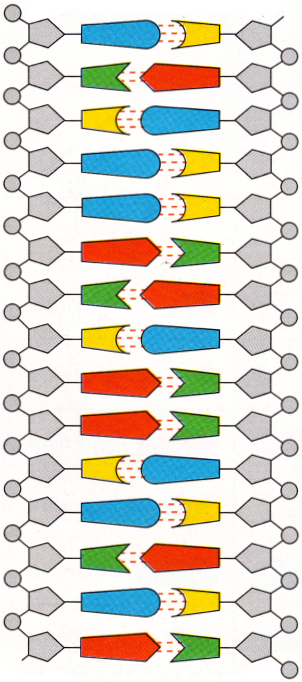
\includegraphics[height=200pt]{bilder/DNA_Schema} %
\end{minipage} %
\end{center} %
\caption{Schematischer Aufbau der DNA. (aus \textit{Lindner Biologie} \citep{Linder}, S. 345/346)}
\label{fig:bio:dna:schema}
\end{figure}

Die Reihenfolge in der diese Nukleobasen (oder einfach kurz Basen) vorkommen, stellen die auf der DNA gespeicherte Information dar. Wie bereits  erwähnt gibt es vier verschiedene Basen, nämlich Adenin, Cytosin, Guanin und Thymin, die jeweils mit ihrem  Anfangsbuchstaben (d.h. A, C, G, T) abgekürzt werden. Eine wichtige Eigenschaft des DNA-Doppelstranges ist die  Komplementarität: Adenin bindet stets an Thymin und Guanin immer an Cytosin. Kennt man also einen Einzelstrang eines DNA-Moleküls, so kann man den fehlenden DNA-Strang rekonstruieren. Adenin und Thymin sind über zwei Wasserstoffbrückenbindungen miteinander verbunden, Cytosin und Guanin mit dreien. Aufgrund ihres chemischen Aufbaus werden Adenin und Guanin als \emph{Purin}-Basen bezeichnet: Sie bestehen aus zwei Kohlenstoff-Stickstoff-Ringen und sind damit ein wenig länger als die \emph{Pyrimidin}-Basen Cytosin und Thymin, die nur aus einem solchen Ring bestehen.

\begin{figure}[htbp]
\begin{center}
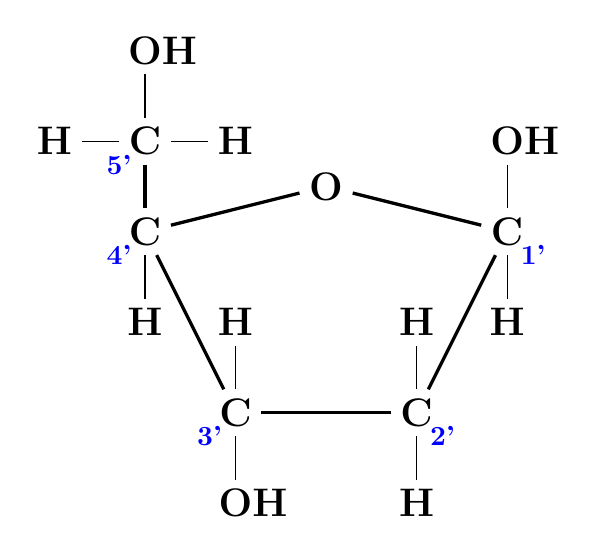
\begin{tikzpicture}
	\pgfmathsetmacro{\normDist}{1.15}
	\tikzstyle{bond}=[very thick]
	\tikzstyle{chem}=[black, font=\bfseries\Large]
	\tikzstyle{num}=[blue, font=\bfseries\normalsize]
	
	\node[chem] (C1) at (2*\normDist, 2*\normDist)	{C};
	\node[chem] (H1a) at (2*\normDist, 3*\normDist)	{\color{white}H\color{black}OH};
	\node[chem] (H1b) at (2*\normDist, 1*\normDist)	{H};	
	
	\node[chem] (C2) at (\normDist, 0)	{C};
	\node[chem] (H2a) at (\normDist, -\normDist)	{H};
	\node[chem] (H2b) at (\normDist, \normDist)	{H};	
	
	\node[chem] (C3) at (-\normDist, 0)	{C};
	\node[chem] (H3a) at (-\normDist, -\normDist)	{\color{white}H\color{black}OH};
	\node[chem] (H3b) at (-\normDist, \normDist)	{H};
	
	\node[chem] (C4) at (-2*\normDist, 2*\normDist)	{C};
	\node[chem] (H4) at (-2*\normDist, 1*\normDist)	{H};	
	
	\node[chem] (C5) at (-2*\normDist, 3*\normDist)	{C};
	\node[chem] (H5a) at (-1*\normDist, 3*\normDist)	{H};	
	\node[chem] (H5b) at (-3*\normDist, 3*\normDist)	{H};	
	\node[chem] (H5c) at (-2*\normDist, 4*\normDist)	{\color{white}H\color{black}OH};	
	
	\node[chem] (O) at (0, 2.5*\normDist)	{O};	

	\draw (C1) -- (H1a);
	\draw (C1) -- (H1b);

	\draw (C2) -- (H2a);
	\draw (C2) -- (H2b);
	
	\draw (C3) -- (H3a);
	\draw (C3) -- (H3b);
	
	\draw (C4) -- (H4);
	
	\draw (C5) -- (H5a);
	\draw (C5) -- (H5b);
	\draw (C5) -- (H5c);
	
	\draw[bond] (C1) -- (C2);
	\draw[bond] (C2) -- (C3);
	\draw[bond] (C3) -- (C4);
	\draw[bond] (C4) -- (C5);
	\draw[bond] (C4) -- (O);
	\draw[bond] (O) -- (C1);
	
	\node[num] at (C1.south east) {1'};
	\node[num] at (C2.south east) {2'};
	\node[num] at (C3.south west) {3'};
	\node[num] at (C4.south west) {4'};
	\node[num] at (C5.south west) {5'};
\end{tikzpicture}
\end{center}
\caption{Chemischer Aufbau der Desoxyribose}
\label{fig:bio:dna:desoxyribose}
\end{figure}

Werfen wir einen genaueren Blick auf das Zuckermolekül der DNA: Die \emph{Desoxyribose}, die der DNA ihren Namen gibt, ist ein Zucker-Molekül, das aus fünf Kohlenstoff-Atomen besteht. Diese C-Atome werden wie in Abbildung \ref{fig:bio:dna:desoxyribose} gezeigt von 1‘ bis 5‘ durchnummeriert. Das erste Kohlenstoff-Atom (1‘) ist mit der Nukleobase (A, C, G oder T) verbunden, wobei beim Verbinden Wasser ($\text{H}_2\text{O}$) abgespalten wird. Beim zweiten C-Atom fällt auf, dass hier die Hydroxy-Gruppe fehlt (-H statt -OH); daher kommt die Vorsilbe "`Desoxy"' im Namen des Zuckermolekül. Am 5‘-Ende des Zuckermoleküls hängt die Phosphatgruppe des Nukleotids. Die Phosphatgruppe eines anderen Nukleotids kann mit dem dritten C-Atom des Zucker-Moleküls verbunden werden, sodass sich Ketten aus Phosphatresten und Zucker-Molekülen bilden. 
%#Formulierung
Hier zeigt sich eine weitere wichtige Eigenschaft der DNA: Die beiden Stränge besitzen jeweils eine Richtung. Man kann die Reihenfolge der Nukleobasen in 3‘-5‘-Richtung lesen oder in 5‘-3‘-Richtung. Analysiert man die Struktur der DNA genauer, stellt man fest, dass die beiden DNA-Stränge eines DNA-Moleküls antiparallel zueinander stehen. Ein Strang liegt in 3‘-5‘-Richtung, der andere in 5‘-3‘-Richtung. 

DNA-Moleküle liegen (wie in Abbildung \ref{fig:bio:dna:doppelhelix} gezeigt) als rechtsläufige Doppelhelix vor. Dabei besteht jede Windung aus etwa 10 Basenpaaren und ist 3,4 nm lang. Die Doppelhelix ist nicht exakt symmetrisch, sondern besteht aus einer großen und einer kleinen Furche. Der Durchmesser eines DNA-Doppelstrangs beträgt ca. 2 nm.

\begin{figure}[htbp]
\begin{center}
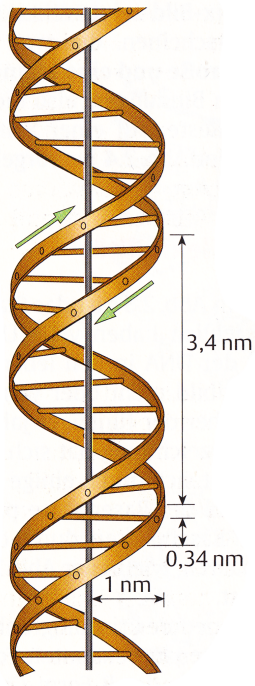
\includegraphics[height=7cm]{bilder/DNA_Helix}
\end{center}
\caption[DNA-Doppelhelix. (aus \citep{Knippers2006}, S. 11)]{DNA-Doppelhelix. Die kleine und große Furche sind deutlich zu erkennen. (aus \citet{Knippers2006}, S. 11)}
\label{fig:bio:dna:doppelhelix}
\end{figure}

\section{Chromosomen}
\label{sec:bio:chromo}
\marginpar{Jens}
DNA-Moleküle können teilweise sehr lang werden, beispielsweise besteht das größte DNA-Molekül des Menschen aus etwa 263 Millionen Basenpaaren. Aus diesem Grund wird die DNA-Doppelhelix um bestimmte Proteine, sogenannte Nukleosomen, herum gewickelt. Durch weitere Proteine wird die DNA weiter zusammengefaltet, wie diese Faltungen jedoch genau aussehen und welche Proteine daran beteiligt sind, ist noch Gegenstand der Forschung \citep{Hansen2012}. 

Der Komplex aus DNA und Proteinen wird als Chromosom bezeichnet. Chromosomen können in drei verschiedenen Formen vorliegen. Kurz vor einer Zellteilung besteht jedes Chromosom aus zwei Chromatinfäden (d.h. zwei DNA-Doppelsträngen), die jeweils dieselbe Information tragen und am \emph{Centromer} miteinander verbunden sind. In schematischen Darstellungen von Chromosomen (wie zum Beispiel Abbildung \ref{fig:bio:chromo:chromosom}) wird fast immer diese Form gezeigt. Während der Zellteilung werden die beiden Chromatinfäden eines Chromosoms auf die beiden Tochterzellen aufgeteilt, sodass das Chromosom nach einer Zellteilung nur noch aus einem Chromatinfaden besteht. Die Chromatinfäden sind während der Zellteilung stark komprimiert und von daher unter einem Lichtmikroskop sichtbar. Zwischen den Zellteilungen liegen die Chromosomen als freies Chromatin vor. Nur in diesem Zustand kann die auf der DNA gespeicherte Information gelesen oder kopiert werden. Unter einem Lichtmikroskop sind die freien, unkomprimierten Chromatinfäden nicht sichtbar.

\begin{figure}[htbp]
\begin{center}
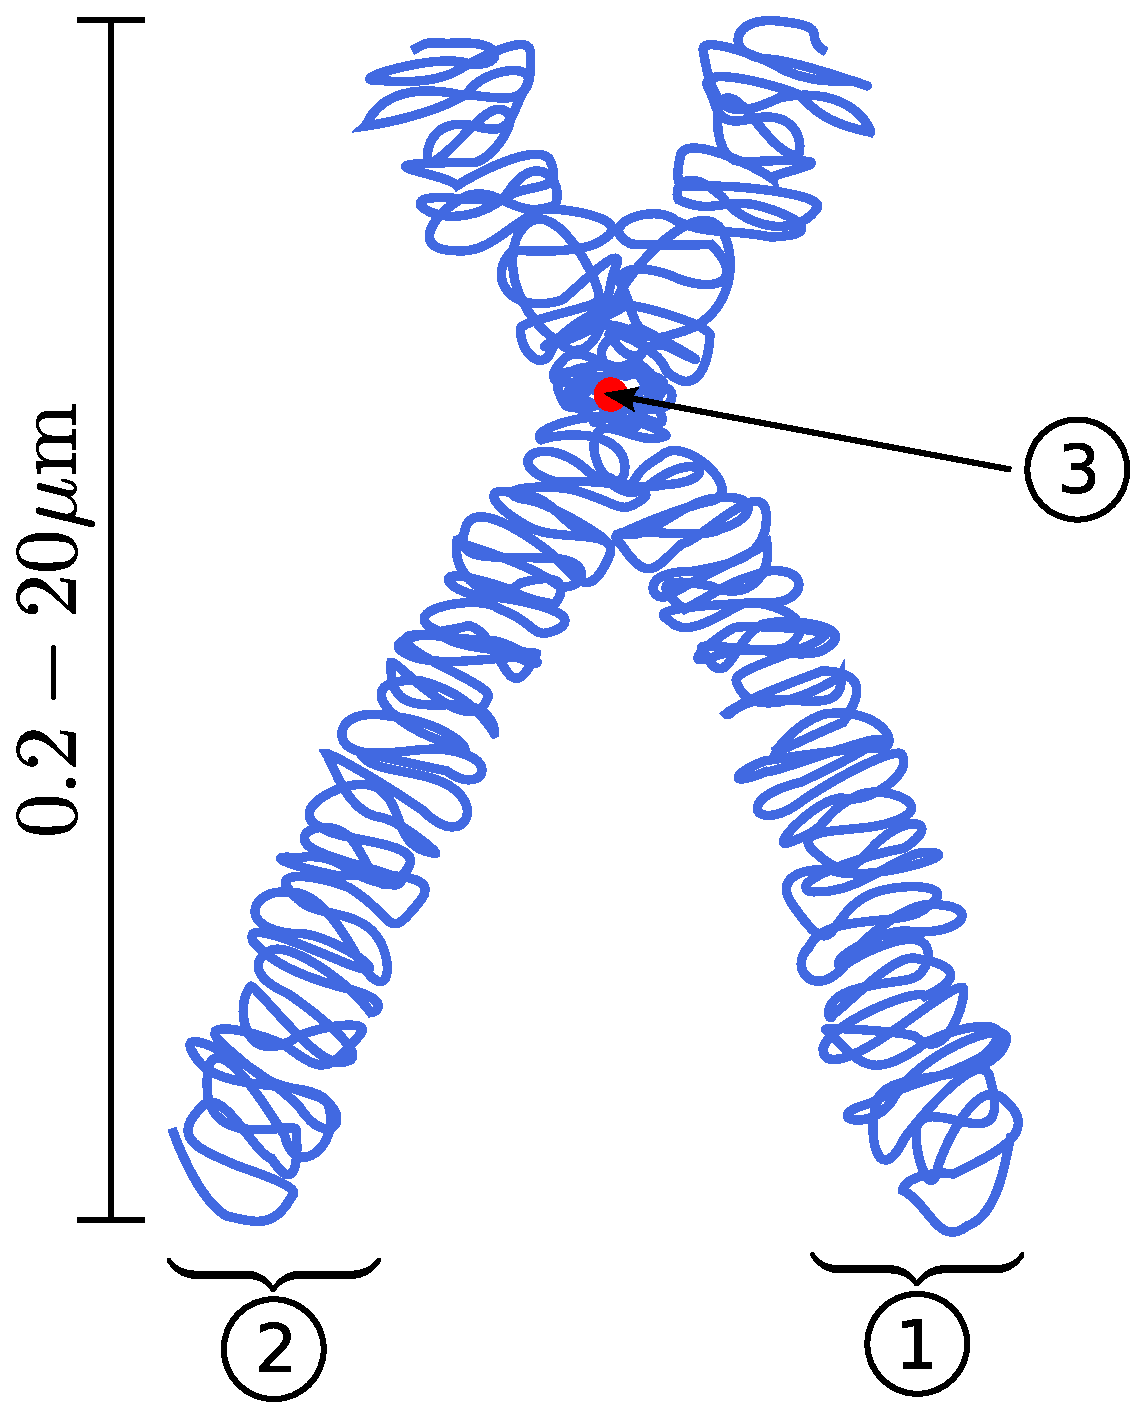
\includegraphics[height=6cm]{bilder/Chromosom}
\end{center}
\caption[Schematische Abbildung eines Chromosoms. (aus \protect\url{http://commons.wikimedia.org/wiki/File:Chromosome.svg})] {Schematische Abbildung eines Chromosoms mit zwei Chromatiden. (1) und (2) die beiden Chromatiden, (3) Centromer. (aus \protect\url{http://commons.wikimedia.org/wiki/File:Chromosome.svg}).}
\label{fig:bio:chromo:chromosom}
\end{figure}

Menschliche Zellen enthalten bis auf wenige Ausnahmen\footnote{Ausnahmen bilden zum einen die Geschlechtszellen, d.h. Spermien bzw. Eizellen (siehe Abschnitt \ref{sec:bio:erb}), sowie Zellen, bei denen sich die Chromosomenzahl durch Krankheiten verändert hat (siehe Abschnitt \ref{sec:bio:muta}).} stets 46 Chromosomen, bzw. 23 Chromosomenpaare. Von jedem Paar haben wir ein Chromosom vom Vater geerbt und eines von der Mutter. Die Informationen, die auf den Chromosomen eines Paares stehen, sind ähnlich, aber nicht zwingend gleich. Das 23. Chromosomenpaar bestimmt das Geschlecht eines Menschen: Frauen haben zwei X-Chromosomen, Männer ein X- und ein Y-Chromosom. Dementsprechend werden diese beiden Chromosomen auch als Geschlechtschromosomen oder kurz Gonosomen bezeichnet. Insgesamt besteht das menschliche Genom (also die Vereinigung aller Chromosomen einer Zelle) aus drei Milliarden Basenpaaren oder kürzer aufgeschrieben 3 Gbp. Die Vorsilbe \emph{G} steht dabei für Giga also $10^9$; \emph{bp} ist die Abkürzung für Basenpaar. Dementsprechend gibt es auch die Einheiten \emph{Mbp} und \emph{kbp} für Millionen bzw. Tausend Basenpaare. Da es für jedes Basenpaar vier Möglichkeiten (A, C, G und T) gibt, beträgt der Informationsgehalt des menschlichen Genoms sechs Milliarden Bit bzw. 750 MB. An dieser Stelle soll nochmal erwähnt werden, dass jede Zelle eines Lebewesens denselben DNA-Code enthält, d.h. jede menschliche Zelle enthält die erwähnten drei Milliarden Basenpaare. 

\begin{figure}[htbp]
\begin{center}
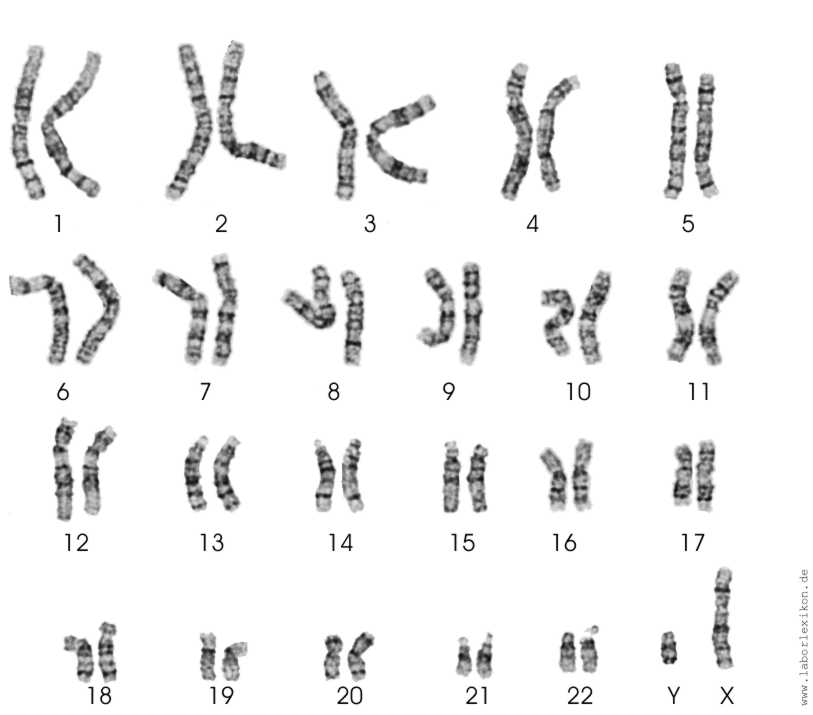
\includegraphics[width=0.8\textwidth]{bilder/Karyogramm}
\end{center}
\caption{Karyogramm des Menschen. (aus \protect\url{http://www.laborlexikon.de/images/Karyogramm-813.JPG})}
\label{fig:bio:chromo:karyogramm}
\end{figure}

\section{Prokaryoten und Eukaryoten}
\label{sec:bio:proeukaryoten}
\marginpar{Jens}

An einigen Stellen ist es wichtig zwischen Pro- und Eukaryoten zu unterscheiden. Eukaryoten sind alle höheren Lebensformen, das heißt Menschen, Tiere, Pflanzen und Pilze. Zu Prokaryoten gehören Bakterien und die Archaebakterien, die auch als Urbakterien bezeichnet werden. Eukaryotische Zellen besitzen die im vorherigen Abschnitt erwähnten Chromosomen, die sich im Zellkern befinden. Prokaryotische Zellen besitzen dagegen keinen Zellkern, ihre DNA ist somit nicht durch eine Membran von den restlichen Zellorganellen abgegrenzt. Des Weiteren enthalten Prokaryoten in der Regel nur ein DNA-Molekül, das ringförmig, also in sich geschlossen ist. 

Da wir uns vor allem mit dem menschlichen Genom beschäftigen, sind für uns hauptsächlich Eukaryoten von Interesse. Trotzdem wird an einigen Stellen erklärt, welche Unterschiede zu Prokaryoten bestehen.

\paragraph{Aufbau einer eukaryotischen Zelle}

Jede Zelle ist von einer Zellmembran umgeben, die die Zelle von der Umgebung abgrenzt. Im Innern der Zellen befinden sich verschiedene, sogenannte Organellen, die bestimmte Funktionen in der Zelle übernehmen. Zu diesen gehört unter anderen der Zellkern, in dem sich die DNA befindet. Das endoplasmatische Retikulum ist mit seinen Ribosomen an der Protein-Biosynthese beteiligt, also an der Übersetzung eines DNA-Abschnitts in ein Protein. In Abschnitt \ref{sec:bio:pbsyn} werden wir mehr dazu erfahren. Der Raum, der zwischen der Zellmembran und den einzelnen Organellen liegt, wird als Zytoplasma bezeichnet. Zellen enthalten noch weitere Organellen, eine Beschreibung dieser würde hier aber zu weit führen. Die Mitochondrien sollen trotzdem kurz erwähnt werden:

\begin{figure}[htbp]
\begin{center}
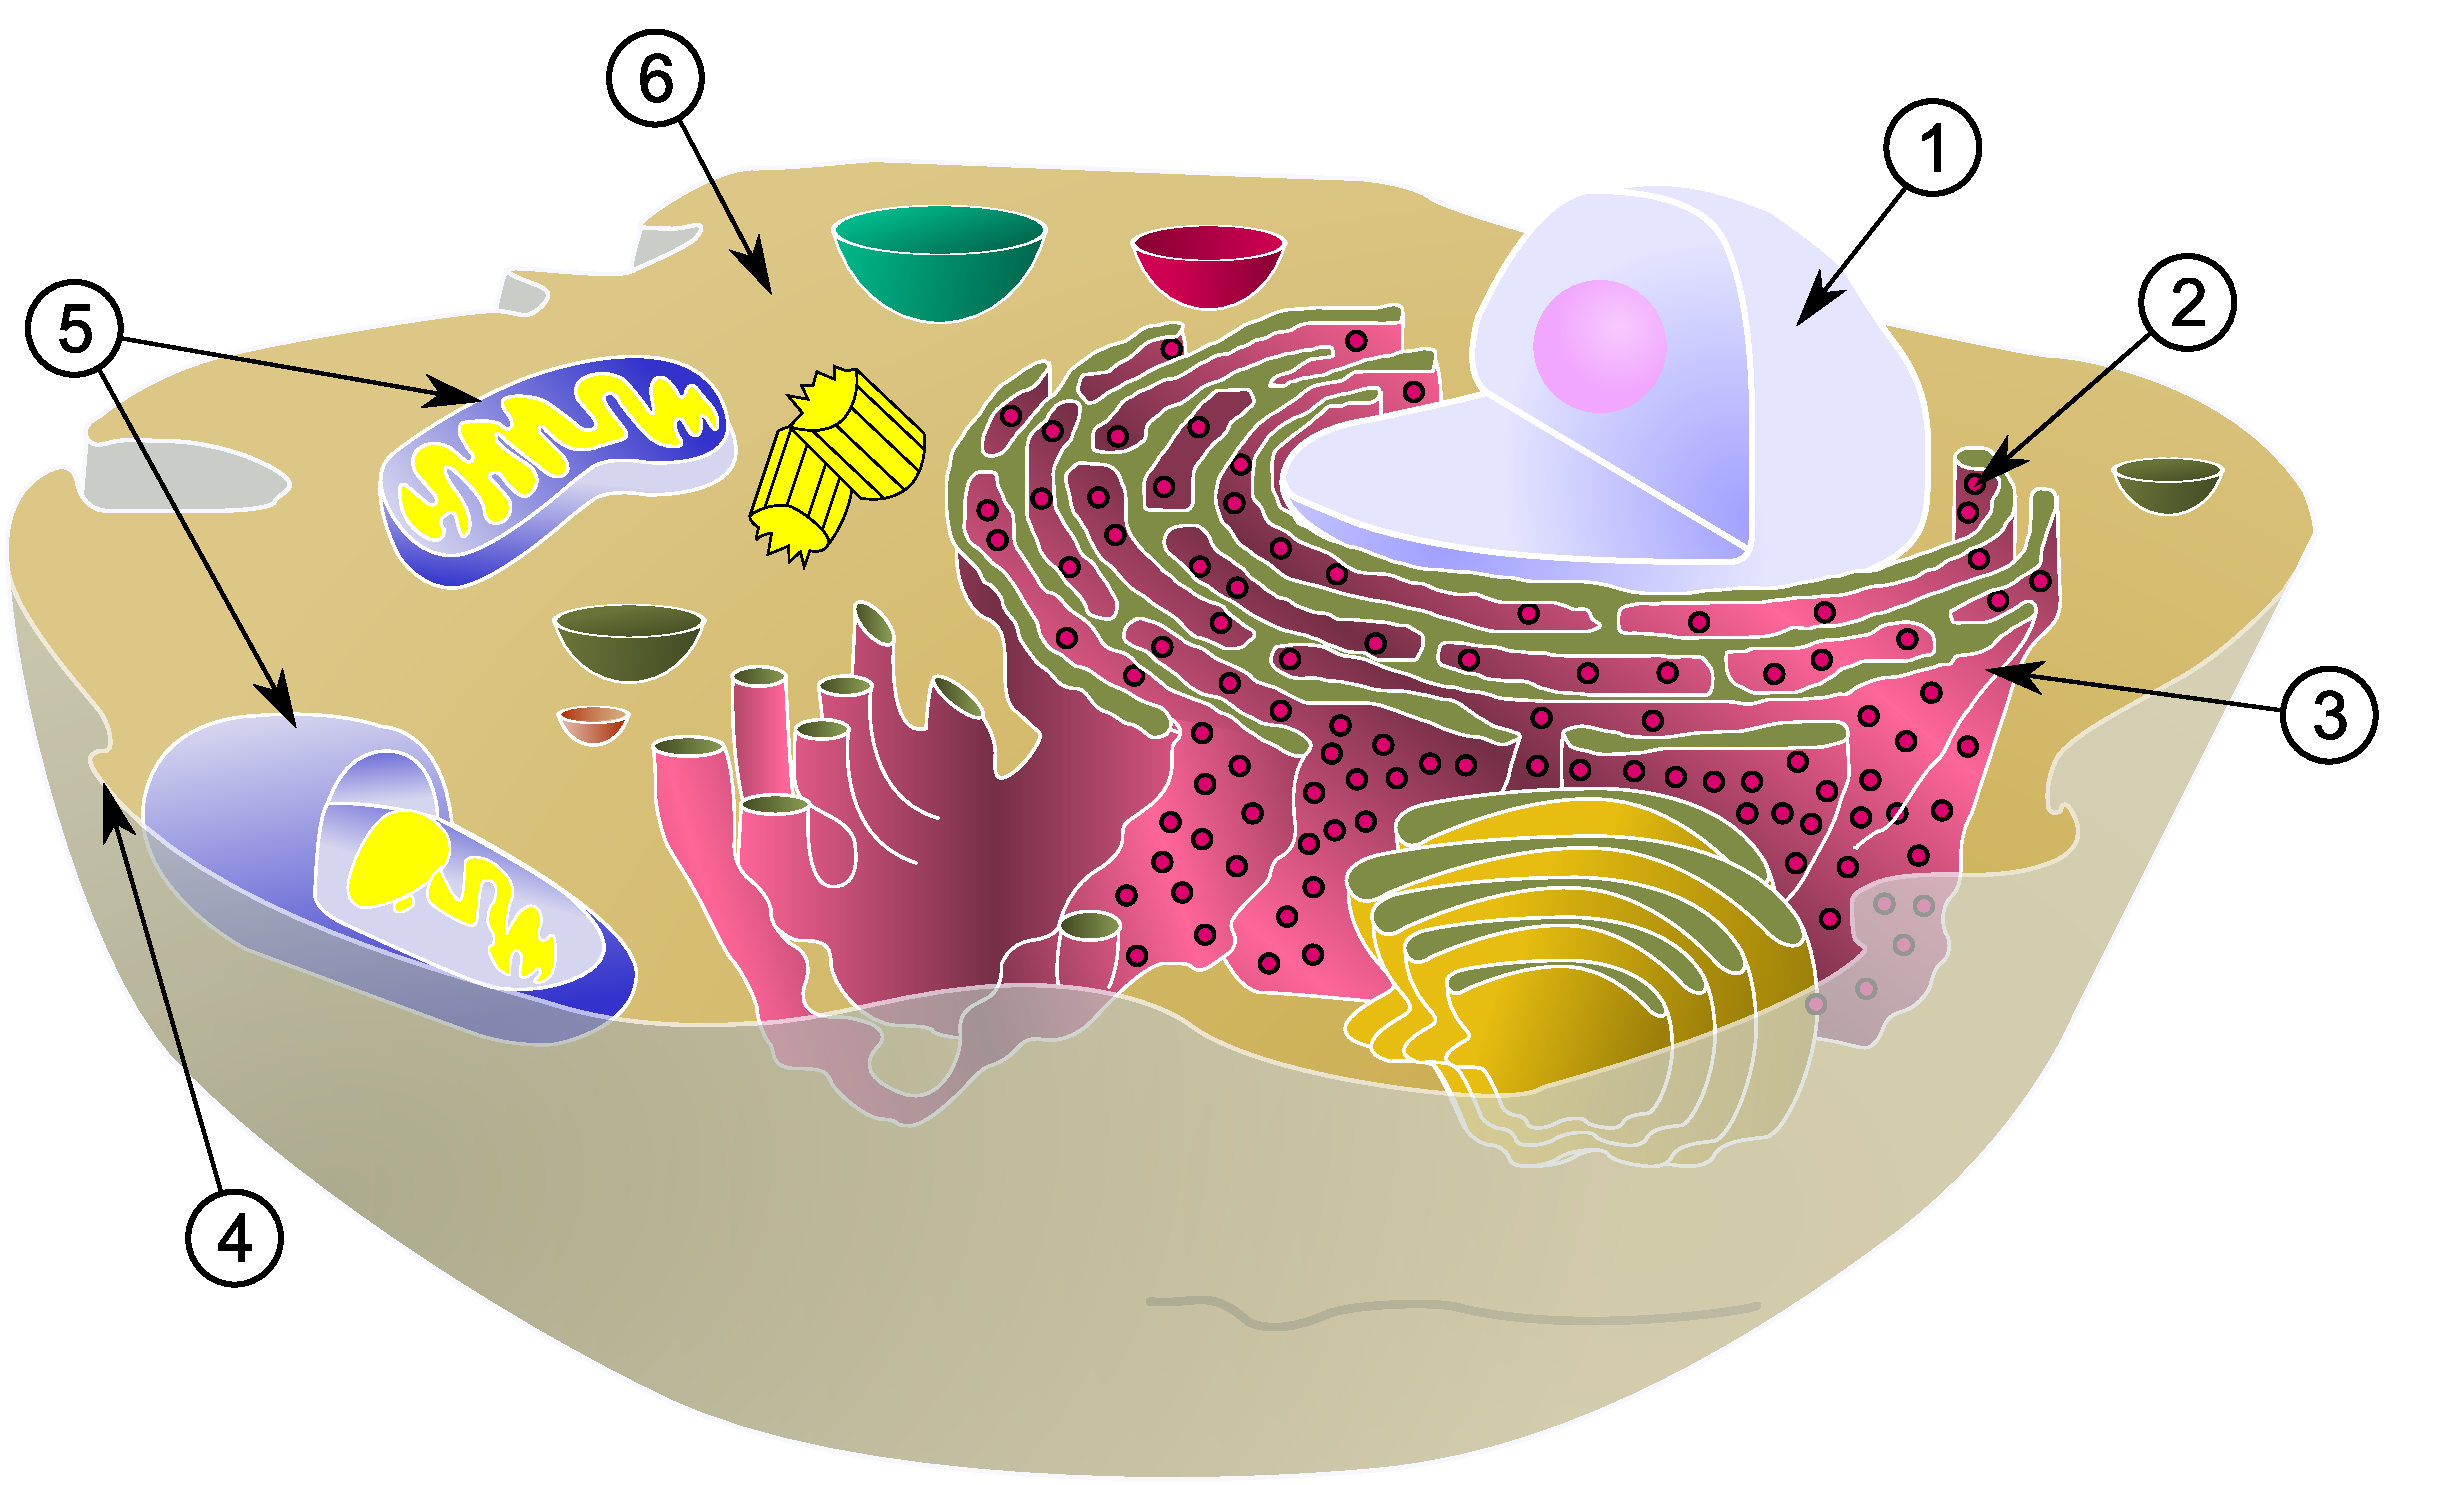
\includegraphics[width=0.95\textwidth]{bilder/Zelle}
\end{center}
\caption[Typische eukaryotische Tierzelle. (aus \protect\url{http://commons.wikimedia.org/wiki/File:Biological_cell.svg})] {Typische eukaryotische Tierzelle. (1) Zellkern, (2) Ribosom, (3) Endoplasmatisches Retikulum, (4) Zellmembran, (5) Mitochondrien, (6) Zytoplasma. (aus \protect\url{http://commons.wikimedia.org/wiki/File:Biological_cell.svg})}
\label{fig:bio:zelle}
\end{figure}

\paragraph{Mitochondrien}

Mitochondrien sind im Prinzip die \textit{Energiekraftwerke} unserer Zellen. Sie stellen Adenosintriphosphat (kurz ATP) her, dass bei sehr vielen Prozessen in unserem Körper als Energieträger genutzt. Wird eine Phosphatgruppe von ATP abgespalten, entsteht Adenosindiphosphat (kurz ADP) und Energie wird frei. Die freiwerdende Energie wird beispielsweise in Muskelzellen als mechanische Arbeit umgesetzt. Auch die für die Herstellung organischer Moleküle benötigte Energie wird durch ATP bereitgestellt. In den Mitochondrien werden ADP und der Phosphatrest wieder zu ATP verbunden. Die dafür nötige Energie liefert zum Beispiel Glucose (Traubenzucker), das direkt oder auch indirekt über die Nahrung aufgenommen wird.

Das in diesem Bericht die Mitochondrien erwähnt werden, hat aber einen anderen Grund: Bisher wurde immer behauptet, dass sich die gesamte DNA einer Zelle im Zellkern befindet. Das ist nicht ganz richtig: Mitochondrien enthalten ebenfalls einen eigenen, kurzen DNA-Ring. Beim Menschen hat dieser DNA-Ring eine Länge von 16.569 Basenpaaren \citep{Mitomap} und enthält zahlreiche überlebenswichtige Gene.

\section{Zellteilung}
\label{sec:bio:zell}
\marginpar{Jens}

Wie bereits erwähnt, enthalten alle Zellen dieselbe DNA-Information. Teilt sich eine Zelle, so muss ihre DNA zunächst verdoppelt werden. Dieser Vorgang wird DNA-Replikation genannt. Anschließend wird bei der Mitose die replizierte DNA auf beide Tochterzellen gleichmäßig aufgeteilt, sodass sich die Zelle teilen kann. Wir schauen uns zunächst die DNA-Replikation an:

\subsection{DNA-Replikation}
\label{sec:bio:zell:repli}
\marginpar{Jens}

Bei der DNA-Replikation, also der Verdopplung der DNA sind eine ganze Reihe an Proteinen beteiligt. Zunächst entwindet die \emph{Topoisomerase} die DNA-Doppelhelix, sodass sie durch die \emph{Helicase} in die zwei Einzelstränge gespalten werden kann. Die eigentliche Replikation wird nun von der \emph{DNA-Polymerase} durchgeführt. Diese liest den DNA-Strang in 3'-5'-Richtung. Dementsprechend wird der neu gebildete DNA-Strang stets am 3'-Ende verlängert.
%
Als Ausgangsmaterial verwendet die DNA-Polymerase \emph{Desoxyribonukleosidtriphosphate} (dNTPs). Diese bestehen aus einem Zuckermolekül (der Desoxyribose), einer der vier Nukleobasen (also Adenin, Cytosin, Guanin oder Thymin) sowie einer Triphosphat-Gruppe. Je nach dem welche Base in dem Molekül verbaut ist, wird dNTP auch als dATP, dCTP, dGTP bzw. dTTP bezeichnet. Bei der DNA-Synthese werden die (zum Original-Strang komplementären) dNTPs unter Abspaltung von Diphosphat miteinander verbunden, sodass sich wieder ein DNA-Doppelstrang mit komplementären Basenpaaren bildet.

Aufgrund der Antiparallelität der DNA (die beiden Stränge eines DNA-Moleküls laufen in entgegengesetzte Richtungen) findet nur beim 3'-5'-Strang eine kontinuierliche Synthese statt. Die Helicase spaltet den DNA-Doppelstrang immer weiter auf, sodass die die DNA-Polymerase beliebig lange weiterarbeiten kann. Der Strang, bei dem die Synthese kontinuierlich stattfindet, wird als Leitstrang bezeichnet. Im Gegensatz dazu findet beim Folgestrang, der in 5'-3'-Richtung verläuft, eine diskontinuierliche Synthese statt. Die DNA-Polymerase arbeitet hier ebenfalls in 3'-5'-Richtung und entfernt sich somit immer weiter von der Helicase. Irgendwann trifft die DNA-Polymerase auf ein bereits repliziertes DNA-Stück, sodass sich die DNA-Polymerase von der DNA löst. Der Bereich zwischen Helicase und bereits verdoppelter DNA wird nun von einer weiteren DNA-Polymerase repliziert, wobei sich diese wiederum von der Helicase entfernt. Es entstehen sogenannte \emph{Okazaki-Fragmente}. Diese werden durch ein weiteres Protein, der \emph{Ligase}, miteinander verbunden, sodass wieder ein ununterbrochener DNA-Doppelstrang vorliegt. 

\begin{figure}[htbp]
\begin{center}
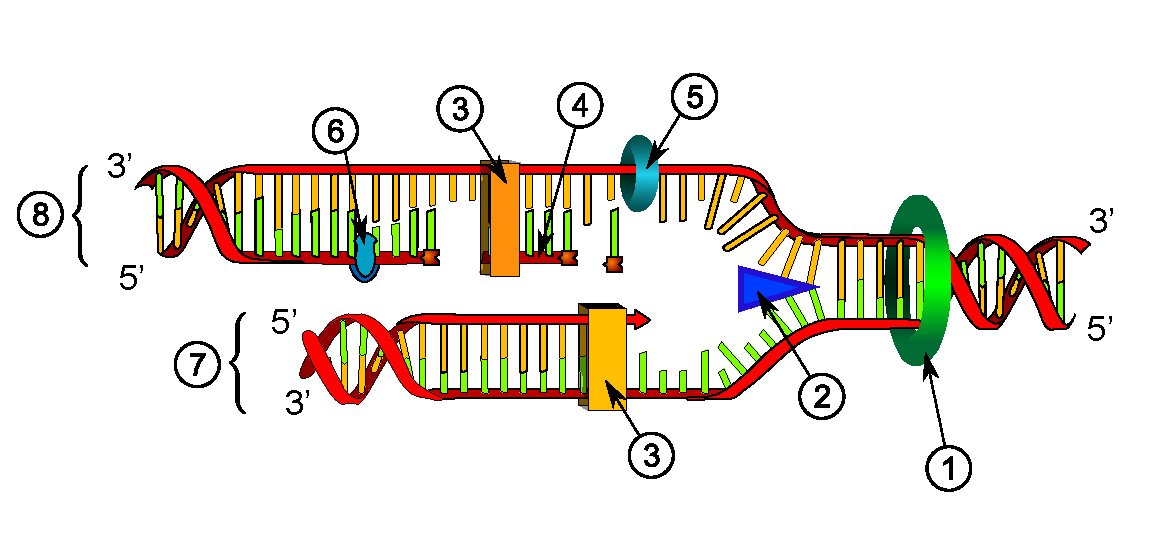
\includegraphics[width=\textwidth]{bilder/DNA_Replikation}
\end{center}
\caption[DNA-Replikation. (aus \protect\url{http://de.wikipedia.org/wiki/Datei:DNA_replication_de.svg})] {DNA-Replikation. (1) Topoisomerase, (2) Helicase, (3) Polymerase, (4) Okazaki-Fragment, (5) Primase, (6) Ligase, (7) Leitstrang (kontinuierliche Synthese), (8) Folgestrang. (aus \protect\url{http://de.wikipedia.org/wiki/Datei:DNA_replication_de.svg})}
\label{fig:bio:zell:repli}
\end{figure}

Aufgrund der Komplementarität der DNA sind die beiden hergestellten Doppelstränge exakte Kopien voneinander. Die neu synthetisierte DNA in 5'-3'-Richtung am Leitstrang entspricht dem originalen 5'-3'-Strang des Folgestranges. Analog dazu gleichen sich auch der alte und neue Strang in 3'-5'-Richtung.

Nach der DNA-Replikation bestehen die Chromosomen aus zwei Chromatiden, die am Centromer miteinander verbunden sind. Die DNA-Doppelstränge in den beiden Chromatiden sind exakte Kopien voneinander. Da die Chromosomen eines Chromosomenpaares ähnliche Informationen enthalten, kann es also sein, dass direkt nach der DNA-Replikation bestimmte Code-Sequenzen in der Zelle in vierfacher Ausführung vorkommen.

\subsection{Mitose}
\label{sec:bio:zell:mitose}
\marginpar{Jens}

Nach der DNA-Replikation findet die eigentliche Zellteilung statt. Hierbei muss die DNA gleichmäßig auf beide Tochterzellen aufgeteilt werden. Dieser Vorgang wird Kernteilung oder in Fachsprache Mitose genannt und besteht aus mehreren Phasen.

In der \emph{Prophase} kondensieren die Chromosomen, sodass sie unter einem Lichtmikroskop sichtbar werden. Sie haben jetzt die kompakte, charakteristische Form mit zwei Chromatiden. Während der \emph{Prometaphase} löst sich die Kernhülle auf. Außerdem wird von den gegenüberliegenden Seiten der Zelle ein Spindelapparat ausgebaut. Die Spindeln heften sich in der \emph{Metaphase} an die Centromere der Chromosomen. In der \emph{Anaphase} werden die beiden Chromatiden der Chromosomen durch den Spindelapparat auseinander gezogen, sodass sich auf beiden Seiten der Zelle 46 Chromosomen mit jeweils einem Chromatid befinden. In der \emph{Telophase} bilden sich dann zwei neue Kernhüllen -- auf jeder Seite der Zelle eine. Gleichzeitig dekondensieren die Chromosomen, d.h. sie breiten sich wieder aus und werden damit unter dem Lichtmikroskop unsichtbar. Die Teilung des Zellkerns ist damit abgeschlossen. 

\begin{figure}[htb]
\begin{center}
\begin{tikzpicture}
	\pgfmathsetmacro{\dst}{3}
	\tikzstyle{textnode}=[font=\bfseries\large];
	\tikzstyle{arr}=[-latex, very thick, shorten >=1ex, shorten <=1ex, bend angle=10, bend left];
	\node (inter) at (-2*\dst, 0)
		{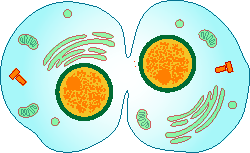
\includegraphics[height=2.8cm]{bilder/Mitose_Interphase}};
	\node (pro) at (-\dst, 1.5*\dst)
		{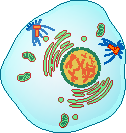
\includegraphics[height=2.8cm]{bilder/Mitose_Prophase}};
	\node (prometa) at (\dst, 1.5*\dst)
		{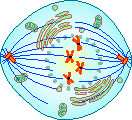
\includegraphics[height=2.8cm]{bilder/Mitose_Prometaphase}};
	\node (meta) at (2*\dst, 0)
		{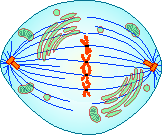
\includegraphics[height=2.8cm]{bilder/Mitose_Metaphase}};
	\node (ana) at (\dst, -1.5*\dst)
		{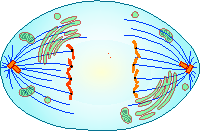
\includegraphics[height=2.8cm]{bilder/Mitose_Anaphase}};
	\node (telo) at (-\dst, -1.5*\dst)
		{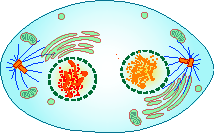
\includegraphics[height=2.8cm]{bilder/Mitose_Telophase}};
		
	\draw[arr] (inter) to (pro);
	\draw[arr] (pro) to (prometa);
	\draw[arr] (prometa) to (meta);
	\draw[arr] (meta) to (ana);
	\draw[arr] (ana) to (telo);
	\draw[arr] (telo) to (inter);
	
	\node[textnode, below=0cm of ana] {Anaphase};
	\node[textnode, below=0cm of telo] {Telophase};
	\node[textnode, above=0.2cm of inter, left] {Interphase};
	\node[textnode, above=0.2cm of meta, right] {Metaphase};
	\node[textnode, above=0cm of prometa] {Prometaphase};
	\node[textnode, above=0cm of pro] {Prophase};
\end{tikzpicture}
\end{center}
\caption{Mitose. (aus \protect\url{http://de.wikipedia.org/wiki/Mitose})}
\label{fig:bio:zell:mitose}
\end{figure}

In der \emph{Interphase}, die in der Regel nicht mehr zur Mitose gezählt wird, teilt sich die Zelle, sodass jede Tochterzelle genau einen Zellkern mit dem vollen Chromosomensatz enthält. Während der Interphase findet auch die Proteinbiosynthese (siehe Abschnitt \ref{sec:bio:pbsyn}) statt, bei der die auf der DNA speicherten Informationen genutzt werden, um Proteine herzustellen. Die Interphase ist also quasi der \textit{normale} Zustand einer Zelle. Vor einer erneuten Zellteilung wird die DNA repliziert. Auch dieser Vorgang gehört zur Interphase.

\subsection{Künstliche DNA-Replikation - PCR}
\label{sec:bio:zell:pcr}
\marginpar{Jens}

Die DNA-Replikation, die vor jeder Zellteilung stattfindet, kann auch künstlich im Reagenzglas durchgeführt werden. Mit Hilfe der Polymerase-Ketten-Reaktion (PCR, engl. Polymerase Chain Reaction) können bereits geringste DNA-Mengen vervielfältigt werden. Zum Erstellen eines genetischen Fingerabdrucks (zum Beispiel bei Mordfällen) werden hinreichend große DNA-Mengen benötigt. Findet man am Tatort beispielsweise eine Hautzelle des Täters, kann die darin enthaltende DNA mit Hilfe der PCR vervielfacht werden. Ohne dieses Verfahren wäre es nicht ohne weiteres möglich, von einer so geringen DNA-Menge einen genetischen Fingerabdruck zu erstellen. Weitere Anwendungen sind Vaterschaftstests oder der Nachweis von Erbkrankheiten. Auch für die Sequenzierung (siehe Abschnitt \ref{sec:bio:seq}), also das Bestimmen der Nukleotid-Abfolge eines DNA-Moleküls, werden hinreichend große DNA-Mengen benötigt. Die PCR ist somit die Grundlage für zahlreiche Anwendungsfälle, bei denen man DNA in hinreichend großer Menge benötigt. 

Die PCR funktioniert dabei folgendermaßen: Zunächst wird die DNA auf 94$^\circ$C erhitzt, wodurch der DNA-Doppelstrang in zwei Einzelstränge gespalten wird (Denaturierung). Bei 70$^\circ$C können sich nun Primer an die DNA lagern. Primer sind kurze DNA-Sequenzen und werden von der DNA-Polymerase als Startpunkte benötigt. Die Wahl der guter Primer ist wichtig, aber auch sehr schwierig: Optimal wäre es, wenn sich die Primer nur an die 3'-Enden der DNA heften, sodass die Polymerase die gesamte DNA vervielfältigen kann. Würden sich die Primer an die Mitte oder gar an das 5'-Ende der DNA lagern, wird ein großer Teil der DNA nicht vermehrt, da die DNA-Polymerase nur in 3'-5'-Richtung arbeitet. Zudem sollte sich nur ein Primer an die jeden DNA-Strang lagern, da sonst bei der Replikation nicht miteinander verbundene Fragmente entstehen.

Nachdem sich die Primer an die DNA gelagert haben, replizieren DNA-Polymerasen die DNA-Stränge. Aus dem ursprünglichen DNA-Doppelstrang entstehen so zwei Kopien. Der beschriebene Zyklus kann beliebig häufig wiederholt werden, wobei natürlich hinreichend viele freie Nukleotide als Ausgangsstoff für die Polymerase vorhanden sein müssen.

Das Erhitzen und Abkühlen übernehmen spezielle Geräte (sogenannte Thermocycler). Sie wiederholen den beschrieben Zyklus der PCR beliebig oft. Da sich bei jeden Schritt die DNA-Menge verdoppelt, steigt die Anzahl der DNA-Kopien exponentiell an: Bereits nach 20 Zyklen liegen theoretisch eine Millionen Kopien vor.

Ein Problem existiert allerdings noch: Bei 94$^\circ$ wird nicht nur die DNA denaturiert, sondern es zersetzen sich auch gewöhnliche DNA-Polymerasen irreversibel. Früher (als die PCR-Methode 1986 eingeführt wurde) wurden tatsächlich nach jeden Zyklus neue Polymerasen zugesetzt. Eine entscheidende Verbesserung lieferte die Taq-Polymerase des Bakteriums \emph{Thermus aquaticus}. Das Bakterium gehört zu den thermophilen, also zu den wärmeliebenden Bakterien und lebt beispielsweise in heißen Quellen oder Geysiren. Seine DNA-Polymerase ist auch noch bei Temperaturen über 94$^\circ$ stabil.

\section{Protein-Biosynthese}
\label{sec:bio:pbsyn}
\marginpar{Jens}


Unter Protein-Biosynthese versteht man die Übersetzung eines DNA-Abschnitts (eines sogenannten Gens) in ein Protein. Dieser Vorgang unterteilt sich in zwei Abschnitte:

Zunächst wird bei der \emph{Transkription} ein Gen der DNA abgelesen und eine RNA-Kopie erstellt. Die Ribonukleinsäure, kurz RNA, ist ähnlich wie DNA aufgebaut, es gibt jedoch drei Unterschiede: Im Gegensatz zur DNA besteht RNA nur aus einem Einzelstrang. Des Weiteren enthält sie als Zuckermolekül -- wie ihr Name bereits vermuten lässt -- die Ribose anstatt der Desoxyribose. Statt der Base Thymin wird in der RNA Uracil verbaut. Chemisch gesehen unterscheidet sich Uracil durch eine fehlende Methyl-Gruppe von Thymin, die möglichen Basenpaarungen sind aber dieselben, d.h. Uracil verbindet sich stets mit Adenin und umgekehrt. Die transkribierte RNA wird auch als messanger-RNA oder kurz mRNA bezeichnet.

Im zweiten Schritt der Proteinbiosynthese wird die mRNA in eine Aminosäure-Sequenz übersetzt. Dieser Vorgang wird als \emph{Translation} bezeichnet. Aminosäure-Sequenzen sind die Vorstufen von Proteinen. 


\subsection{Transkription}
\label{sec:bio:pbsyn:transkription}
\marginpar{Jens}


Bei der Transkription erstellt ein bestimmter Protein-Komplex, die sogenannte  RNA-Polymerase, eine mRNA-Kopie eines DNA-Abschnitts. Dieser Vorgang kann in drei Phasen unterteilt werden:

Bei der \emph{Initiation} setzt sich eine RNA-Polymerase an den Promotor eines Gens. Der Promotor ist eine spezielle DNA-Sequenz, die Informationen darüber enthält, wann und in welchen Zelltyp ein Gen transkribiert soll. Der Promotor codiert somit selbst kein Protein, sondern reguliert die Genexpression. Diese Regulation ist sehr wichtig, da jede Zelle dieselbe DNA-Information enthält. Eine Magenzelle muss beispielsweise ganz andere Proteine herstellen als eine Nervenzelle im Gehirn.

In der zweiten Phase, der \emph{Elongation}, wird die DNA von der RNA-Polymerase in 3'-5'-Richtung abgelesen und eine komplementäre mRNA-Kopie erstellt. Die Synthese der RNA erfolgt somit in 5'-3'-Richtung. 

Nachdem das Gen abgelesen wurde, löst sich die RNA-Polymerase vom DNA-Strang. Dieser Vorgang wird das \emph{Termination} bezeichnet, es ist allerdings noch ungeklärt, wann die Termination genau stattfindet bzw. wodurch sie eingeleitet wird. 


\subsection{Proteine}
\label{sec:bio:pbsyn:proteine}
\marginpar{Jens}
Bevor wir uns der Translation widmen, bei der die mRNA in ein Protein übersetzt wird, wollen wir zunächst klären, was überhaupt Proteine sind: Proteine bestehen aus Aminosäuren, von denen 20 verschiedene in der Natur vorkommen (siehe Abbildung \ref{fig:bio:pbsyn:amino}). Aminosäuren können miteinander verbunden werden und bilden dann Aminosäure-Sequenzen, die auch als Polypeptide bezeichnet werden. Proteine können aus mehren solcher Polypeptide bestehen, wobei die Faltung der Aminosäuren-Sequenzen für die Funktion entscheidend ist.

\begin{figure}[htbp]
\begin{center}
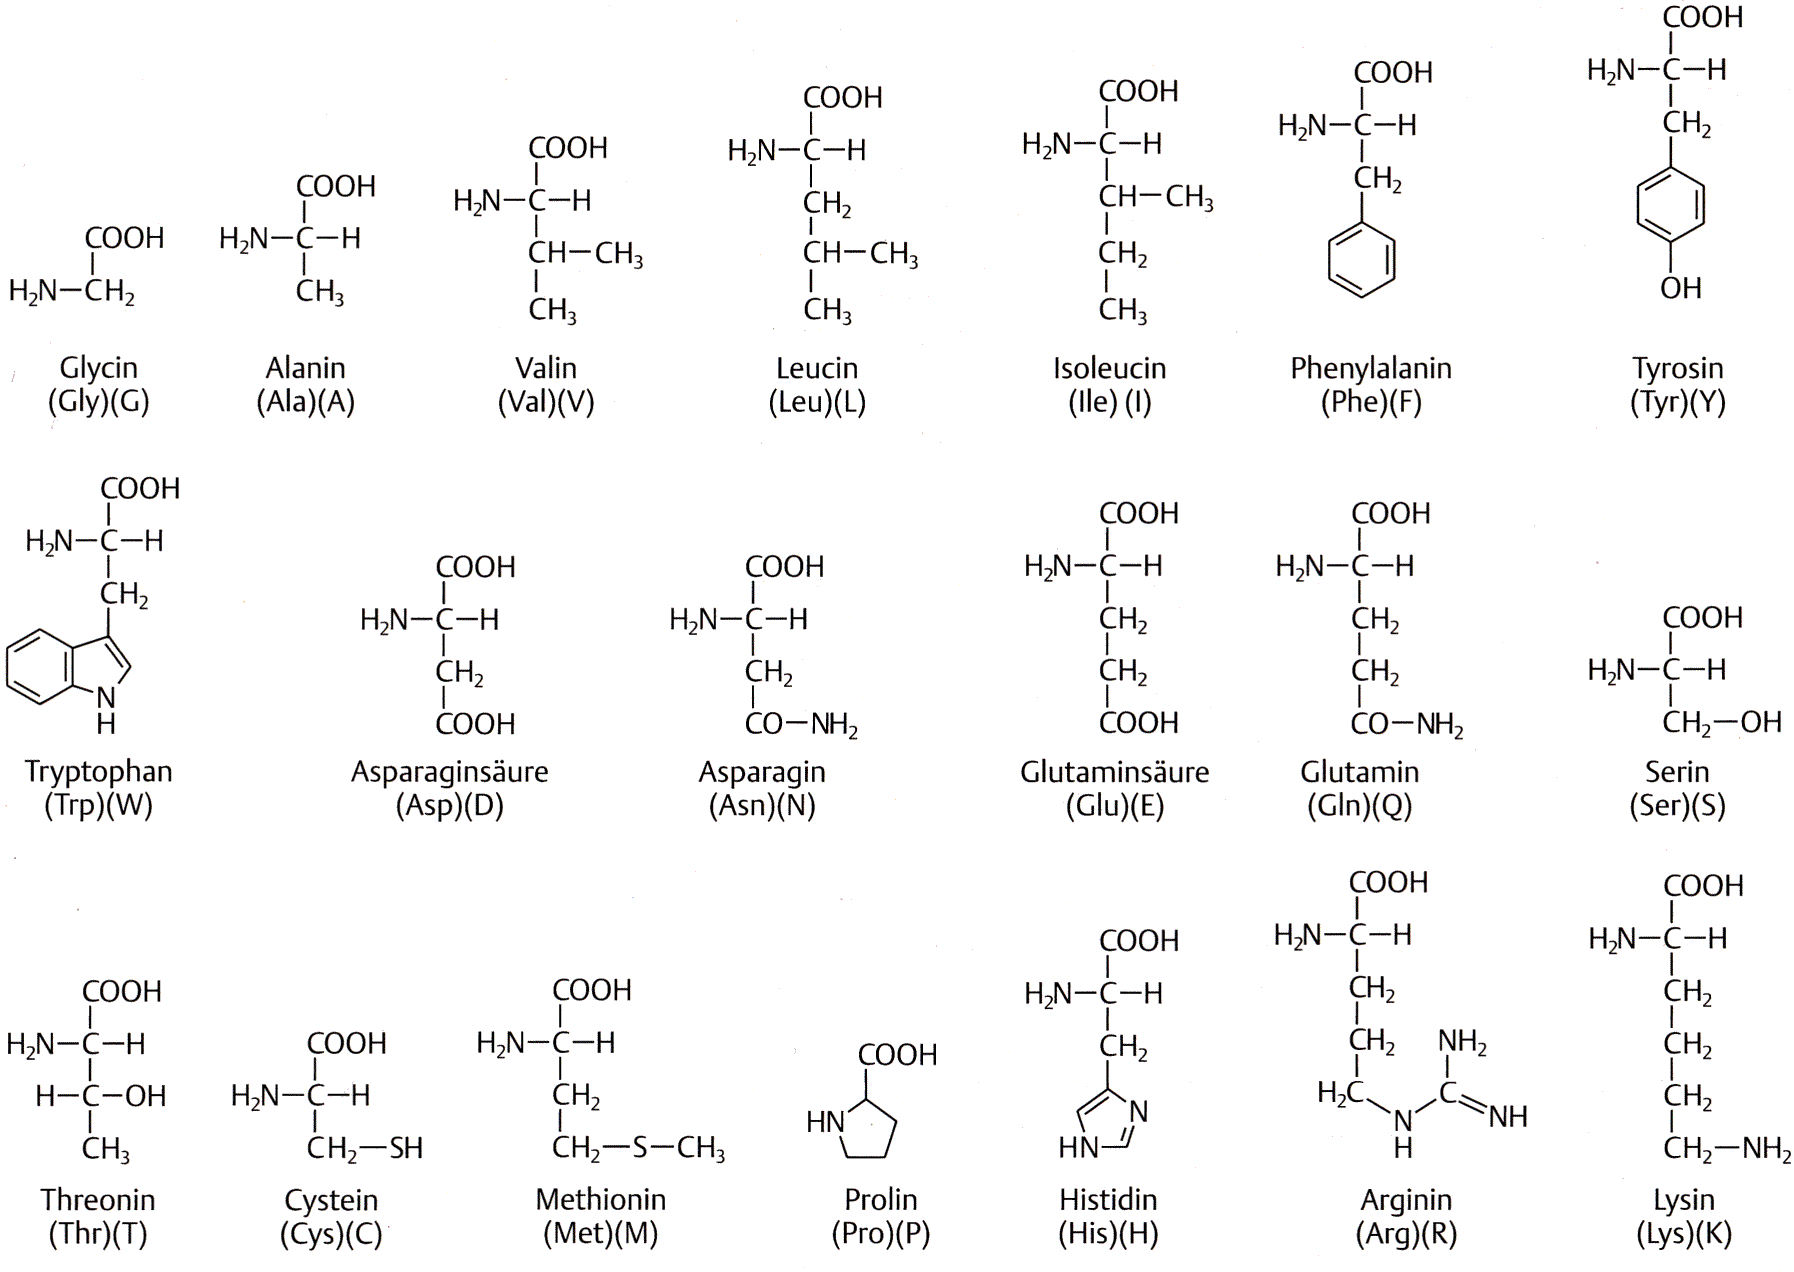
\includegraphics[width=0.8\textwidth]{bilder/Aminoacids}
\end{center}
\caption{Übersicht der 20 natürlich vorkommenden Aminosäuren. (aus \citet{Knippers2006}, S. 38)}
\label{fig:bio:pbsyn:amino}
\end{figure}

Proteine können die unterschiedlichsten Aufgaben im Organismus übernehmen: Das Protein Hämoglobin sorgt beispielsweise in unserem Blut dafür, dass Sauerstoff von den Lungenbläschen zu den Zellen transportiert wird. Proteine, die als Katalysator für chemische Reaktionen dienen, werden auch Enzyme genannt. Als Beispiel könnte man Lactase nennen, ein Enzym, dass Milchzucker (Lactose) in Galactose und Glucose (Traubenzucker) spaltet. Es gibt noch viele weitere Funktionen, die Proteine erfüllen können, beispielsweise als Ionen-Kanal in der Zellmembran.

Die Aminosäuren aus denen Proteine bestehen werden häufig mit drei Buchstaben abgekürzt (z.B. Gly für Glycin, Ala für Alanin, usw.). Darüber hinaus gibt es einen Ein-Buchstaben-Code, die verwendeten Buchstaben überschneiden sich aber mit den Abkürzungen für die Nukleobasen in DNA und RNA. So wird beispielsweise die Aminosäure Glycin ebenso mit G abgekürzt wie auch die Base Guanin.




\subsection{Translation}
\label{sec:bio:pbsyn:translation}
\marginpar{Jens}

Unter Translation versteht man die Übersetzung der mRNA in ein Protein. Die Translation der Eukaryoten unterscheidet sich von der Translation der Prokaryoten. Bei Prokaryoten (d.h. Bakterien und Archaebakterien) findet die Translation noch während der Transkription statt. Bei Eukaryoten ist die Translation räumlich von der Transkription getrennt. Außerdem findet bei Eukaryoten eine Nachverarbeitung der mRNA statt. Dieser Vorgang wird Prozessierung genannt und in Abschnitt \ref{sec:bio:pbsyn:prozess} genauer erklärt. Nach der Prozessierung verlässt die reife mRNA durch eine Kernpore den Zellkern. Die eigentliche Translation läuft dann ähnlich wie bei Prokaryoten ab und soll nun genauer erklärt werden.

Wie bereits erwähnt, codiert ein mRNA-Strang eine Aminosäure-Sequenz. Es gibt jedoch 20 verschiedene Aminosäuren, aber nur vier verschiedene Basen (A, C, G und U) in der mRNA. Aus diesem Grund bilden immer drei Basen ein sogenanntes Codon und codieren eine Aminosäure. In der Code-Sonne (siehe Abbildung \ref{fig:bio:pbsyn:codesonne}) können wir ablesen, welche Basentripletts welche Aminosäure codieren.


\begin{figure}[htb]
\begin{center}
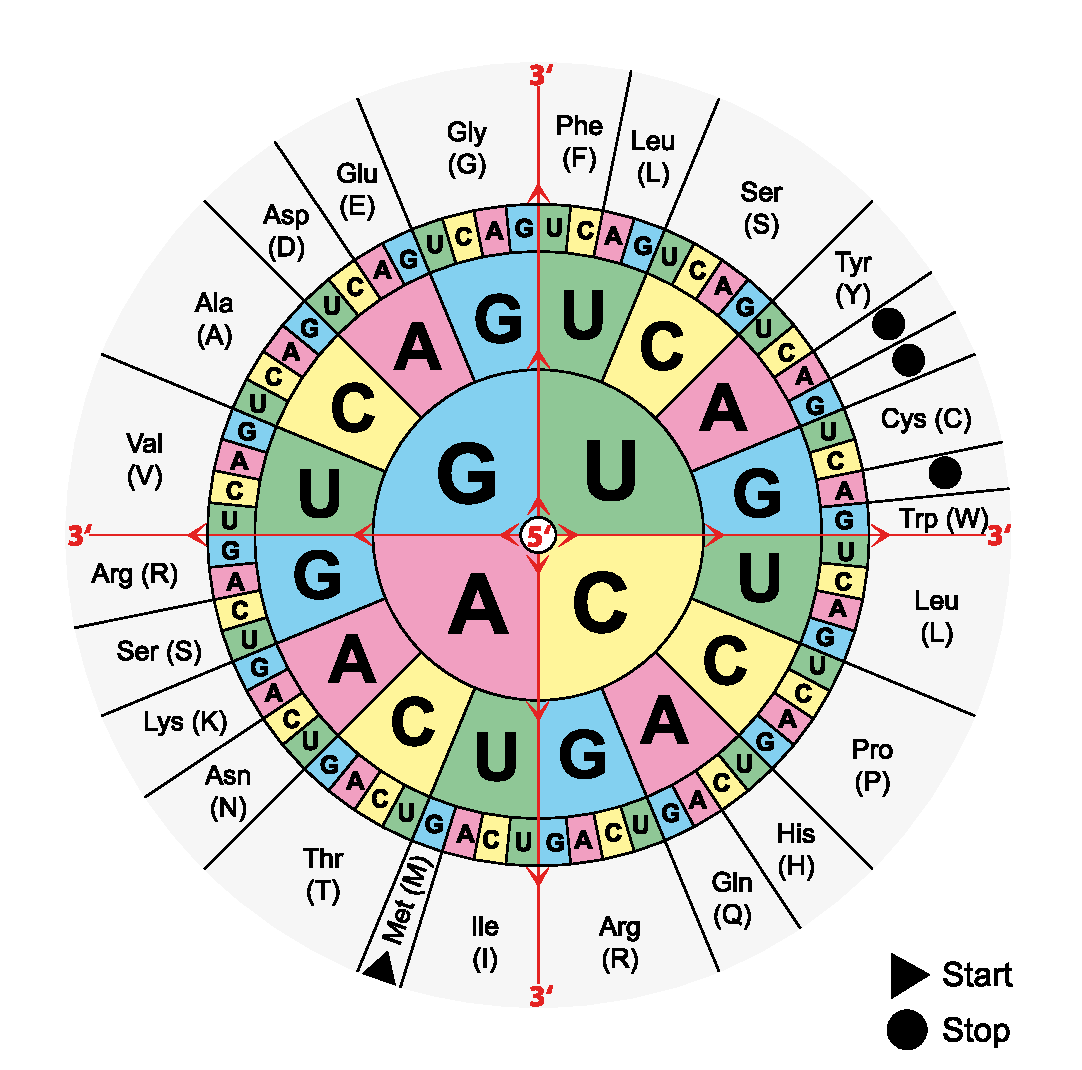
\includegraphics[width=0.7\textwidth]{bilder/Genetischer_Code}
\end{center}
\caption[Genetischer Code. (aus \protect\url{http://commons.wikimedia.org/wiki/File:Aminoacids_table.svg})]{Genetischer Code. Die Basentripletts der mRNA in 5'-3'-Richtung werden (von innen nach außen gelesen) in die gezeigten Aminosäuren übersetzt. (aus \protect\url{http://commons.wikimedia.org/wiki/File:Aminoacids_table.svg})}

\label{fig:bio:pbsyn:codesonne}
\end{figure}

Die Translation findet in 5'-3'-Richtung statt, dementsprechend wird die Code-Sonne von innen nach außen gelesen. Die in der Code-Sonne gezeigte Übersetzung von Codons in Aminosäuren wird auch als genetischer Code bezeichnet.

Die Translation übernehmen die Ribosomen einer Zelle. Sie verbinden sich mit dem mRNA-Strang und lesen ihn solange, bis sie auf das Startcodon AUG treffen. Erst jetzt wird mit der eigentlichen Translation begonnen. Transfer-RNA-Moleküle (kurz tRNA) transportieren je eine Aminosäuren zum Ribosomen. Dazu besitzt die tRNA ein zum entsprechenden Codon komplementäres Anticodon, wobei für jede Aminosäure mindestens eine tRNA existiert. tRNA ist eine besondere Form der RNA: Sie besitzt teilweise Doppelstrangstrukturen und Schleifen, sowie spezielle modifizierte Basen. Im Ribosom verbindet sich das Codon der mRNA mit dem Anticodon einer passenden tRNA. Das Ribosom fügt die von der tRNA transportierte Aminosäure an die aktuelle Aminosäure-Sequenz an. Dieser Vorgang wird so lange durchgeführt, bis das Ribosom auf eines der drei möglichen Stopp-Codons trifft (UAA, UAG und UGA). Hier endet die Translation und das fertige Polypeptid löst sich vom Ribosom. Typischerweise bestehen Proteine aus 100 bis 800 Aminosäuren, es gibt aber auch weitaus größere Proteine.  

\subsection{Prozessierung}
\label{sec:bio:pbsyn:prozess}
\marginpar{Jens}

Bei Eukaryoten findet zwischen Transkription und Translation eine Nachverarbeitung der mRNA statt. Bei diesem Vorgang, den man auch als Prozessierung bezeichnet, wird die sogenannte \emph{prä-mRNA} in \emph{reife mRNA} umgewandelt. Dabei passiert folgendes:

%Bei Eukaryoten findet im Zellkern eine Nachverarbeitung der gerade transkribierten mRNA statt. Vor dieser Nachverarbeitung wird die mRNA auch \emph{prä-mRNA} genannt und nach dieser \emph{reife mRNA}. Bei dieser Nachverarbeitung, die auch Prozessierung genannt wird, passiert folgendes:

Im Gegensatz zu Prokaryoten (bei denen die Translation noch während der Transkription stattfindet) muss die mRNA bei Eukaryoten zwischen Transkription und Translation einen weiten Weg zurücklegen. Zellen enthalten Enzyme, die versuchen jegliche mRNA abzubauen. Um die prä-mRNA davor zu schützen wird ein zusätzliches, modifiziertes Guanin-Nukleotid am 5'-Ende angebracht. Dieser Vorgang wird als \emph{Capping} bezeichnet. Auch die \emph{Polyadenylierung}, bei der das 3'-Ende der mRNA mit Adenin-Nukleotiden verlängert wird, dient der Verhinderung des vorzeitigen Abbaus. Für uns sind aber vor allem das Splicing und RNA-Editing interessant, bei der die codierenden Bereiche der prä-mRNA nachträglich verändert werden.

\paragraph{RNA-Editing}
Beim RNA-Editing werden einzelne Basen der mRNA verändert, sodass zum Beispiel andere Aminosäuren im Protein verbaut werden. Dadurch unterscheidet sich die reife mRNA von der komplementären DNA-Vorlage. Als Beispiel für RNA-Editing sei das Apolipoprotein B genannt. Dieses kommt in zwei verschiedenen Formen in unserem Körper vor: In Leberzellen in der langen Form mit 4536 Aminosäuren, in Dünndarmzellen in der kurzen Form mit 2153 Aminosäuren. Beide Formen entstehen aus derselben prä-mRNA und damit aus demselben DNA-Abschnitt. Die Ursache für die zwei verschiedenen Formen ist das erwähnte RNA-Editing. In den Dünndarmzellen wird an einer bestimmten Stelle in der prä-mRNA Cytosin in Uracil umgewandelt. Dadurch entsteht ein Stopp-Codon, sodass eine entsprechend kürzere Aminosäure-Sequenz gebildet wird. 

RNA-Editing kommt bei Eukaryoten sehr häufig vor. Teilweise werden hierbei auch spezielle Basen (wie zum Beispiel Inosin) verbaut. Solche speziellen Basen kommen zum Beispiel an vielen Stellen der tRNA vor.

\paragraph{Splicing}
Unter Splicing versteht man der Herausschneiden bestimmter Bereiche der prä-mRNA. Die prä-mRNA besteht aus Exons und Introns. Die Introns werden beim Spleißen herausgeschnitten. Die übrigen Abschnitte codieren Proteine und werden Exons genannt.

Beim \emph{alternativen Splicing} kann eine prä-mRNA auf verschiedene Weisen gespleißt werden. Beispielsweise kann es vorkommen, dass in manchen Zellen bestimmte Exons übersprungen oder andere Exons eingebaut werden. Eine weitere Möglichkeit sind alternative Spleißstellen. Hierbei wird nur ein Teil eines Exons übersprungen. Abbildung \ref{fig:bio:pbysn:splicing} veranschaulicht die verschiedenen Möglichkeiten des alternativen Splicings. Ein Gen (also ein DNA-Abschnitt) kann somit wie beim RNA-Editing verschiedene Proteine codieren. 

\begin{figure}[htbp]
\begin{center}
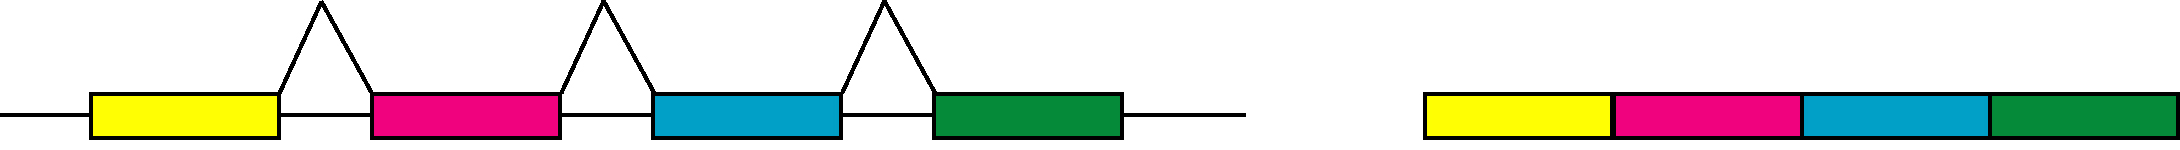
\includegraphics[width=0.7\textwidth]{bilder/Splicing_1} \\
Gewöhnliches Splicing \\
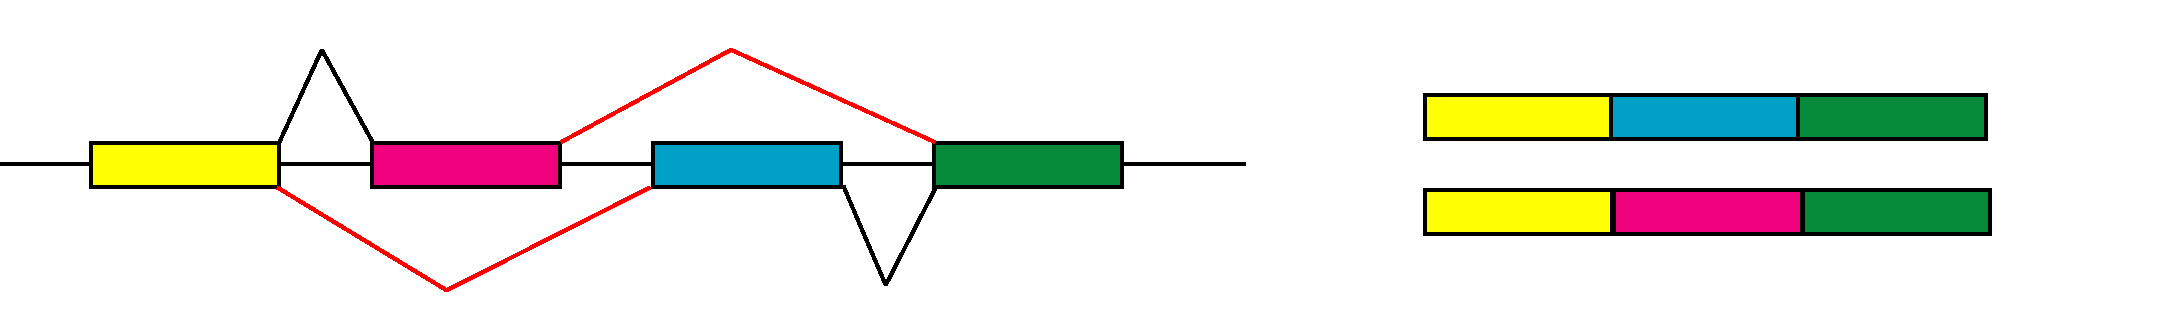
\includegraphics[width=0.7\textwidth]{bilder/Splicing_4} \\
Überspringen von Exons \\
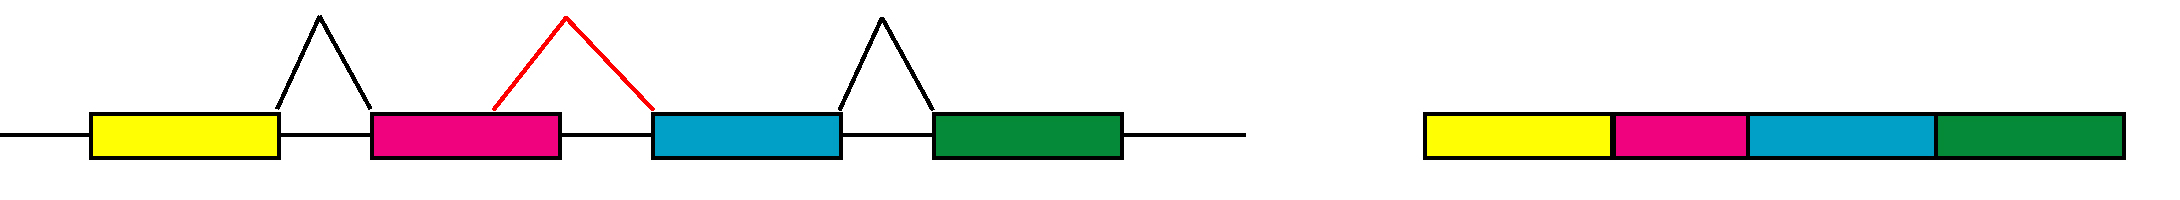
\includegraphics[width=0.7\textwidth]{bilder/Splicing_5} \\
Alternative 5'-Spleißstelle \\
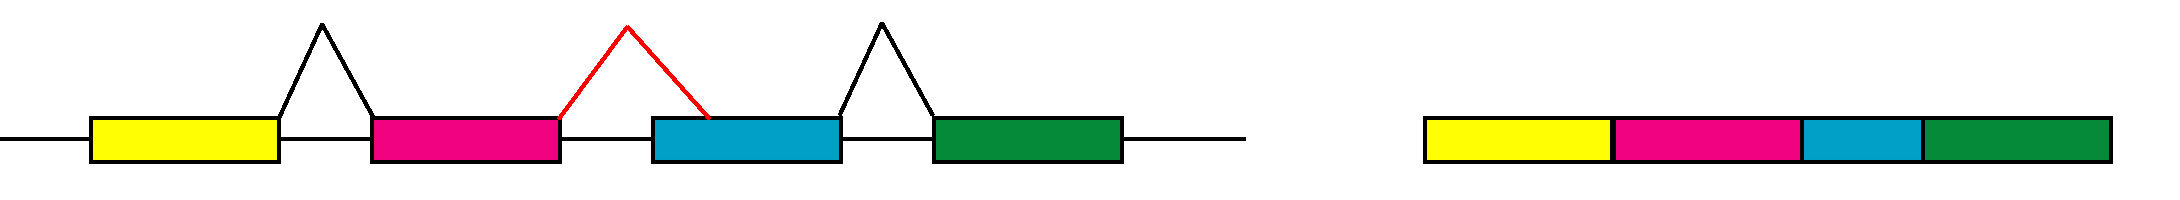
\includegraphics[width=0.7\textwidth]{bilder/Splicing_6} \\
Alternative 3'-Spleißstelle
\end{center}
\caption[Alternatives Splicing (aus \protect\url{http://commons.wikimedia.org/wiki/File:Alternative_splicing.jpg})]{Verschiedene Möglichkeiten beim alternativen Splicing. (aus \protect\url{http://commons.wikimedia.org/wiki/File:Alternative_splicing.jpg})}
\label{fig:bio:pbysn:splicing}
\end{figure}

\section{Vererbung}
\label{sec:bio:erb}
\marginpar{Jens}

Die auf der DNA enthaltene Information wird an die Nachkommen weitervererbt. Dabei ergibt sich jedoch folgendes Problem: Würden Vater und Mutter jeweils ihre 46 Chromosomen weitervererben, so hätte das Kind 92 Chromosomen. Mit jeder weiteren Generation würde sich die Chromosomenzahl erneut verdoppeln. Aus diesem Grund besitzen Eizellen und Spermien nur einen haploiden Chromosomensatz, der aus 23 Chromosomen besteht, und zwar von jedem Chromosomenpaar genau eines. Alle anderen Zellen unseres Körper sind diploid und besitzen somit 46 Chromosomen. Die Halbierung der Chromosomenzahl findet bei der Meiose statt und soll hier nur kurz erläutert werden soll:
\newpage

\subsection{Meiose}
\label{sec:bio:erb:meiose}
\marginpar{Jens}

Zu Beginn der Meiose findet eine Replikation der DNA statt, sodass die Chromosomen der Zelle aus zwei Chromatiden bestehen. Während der ersten Reifeteilung baut sich ähnlich wie bei der Mitose ein Spindelapparat aus. Im Unterschied zur Mitose werden aber nicht die Schwester-Chromatiden voneinander getrennt, sondern die homologen Chromosomen (d.h. die beiden Chromosomen eines Chromosomenpaares). Nachdem sich die Zelle geteilt hat, liegen zwei Zellen mit haploiden Chromosomensatz vor, deren Chromosomen aber immer noch aus zwei Chromatiden bestehen. Bei der zweiten Reifeteilung werden nun analog zur Mitose die Chromatiden voneinander getrennt, sodass letztendlich vier haploide Zellen mit 1-Chromatid-Chromosomen vorliegen.

Während der ersten Reifeteilung kann ein Crossing-Over stattfinden. Dabei werden DNA-Sequenzen zwischen den homologen Chromosomen ausgetauscht. Die Chromosomen eines Kindes sind somit keine exakten Kopien der Chromosomen der Großeltern. Durch das Crossing-Over erhöht sich die genetische Vielfalt, was für das Überleben einer Art sehr vorteilhaft sein kann.

\subsection{Grundbegriffe der Vererbungslehre}
\marginpar{Jens}

Der Begriff Gen wurde bisher schon mehrfach benutzt, allerdings noch nicht genau definiert. Eine eindeutige Definition ist schwierig zu formulieren, fest steht aber, dass es sich bei einem Gen um einen Abschnitt auf DNA handelt. Im Laufe der Geschichte gab es viele Versuche, den Begriff Gen festzulegen. Nach der Entdeckung der DNA-Struktur (1953) wurde ein Gen als ein Abschnitt auf der DNA gesehen, der die Information zur Herstellung eines Proteins trägt. Jedoch insbesondere bei Eukaryoten codiert ein und derselbe DNA-Abschnitt häufig verschiedene Proteine. Wir haben dies bereits beim RNA-Editing und beim alternativen Spleißen kennen gelernt (siehe Abschnitt \ref{sec:bio:pbsyn:prozess}). Darüber hinaus gibt es DNA-Abschnitte, die zur Herstellung der Transfer-RNA oder anderer besonderer RNA dienen (siehe Abschnitt \ref{sec:bio:pbsyn:translation}). Aus diesem Grund, wird heutzutage ein Gen als ein DNA-Abschnitt definiert, der die Information zur Herstellung einer biologisch aktiven RNA enthält. Dabei kann es sich um mRNA handeln, die später in ein Protein übersetzt wird, aber auch um andere RNA-Typen, wie zum Beispiel die erwähnte tRNA. 

Gene können in zwei oder mehr unterschiedlichen Ausbildungsformen vorliegen, die als \emph{Allele} bezeichnet werden. Unter \emph{Genotyp} verstehen wir die Gesamtheit der Gene eines Individuums, unter \emph{Phänotyp} sein äußeres Erscheinungsbild. \emph{Dominante} Allele wirken bei der Ausbildung des Phänotyps bestimmend und unterdrücken \emph{rezessive} Allele in ihrer Wirkung. 

Ein Beispiel soll die gerade genannten Begriffe verdeutlichen. Beim Menschen gibt es vier verschiedene Blutgruppen, die sich anhand der gebildeten Blutgruppensubstanz unterschieden. Bei Blutgruppe A wird die Substanz A gebildet, bei Blutgruppe B die Substanz B, bei AB beide Substanzen, bei 0 keine von beiden. Ursache für die verschiedenen Blutgruppen sind drei Allele eines Gens. Das Allel $i^A$ codiert die Blutgruppensubstanz A, $i^B$ die Substanz B. Beim Allel $i$ wird keine Blutgruppensubstanz gebildet. Die Allele $i^A$ und $i^B$ wirken dominant. Wenn sie vorliegen, wird immer die jeweilige Substanz gebildet. Das rezessive Allel $i$ kommt nur zur Wirkung, wenn kein dominantes Allel vorhanden ist. Da jedes Gen in zweifacher Ausführung vorkommt (nämlich auf den beiden homologen Chromosomen eines Paares), besitzen wir immer zwei Allele. Eines haben wir von der Mutter geerbt, das andere vom Vater. Nun können wir den verschiedenen Phänotypen (also den Blutgruppen) die  möglichen Genotypen zuordnen. Bei Blutgruppe 0 müssen beide Allele vom Typ $i$ sein. Der Genotyp ist also $ii$. Bei Blutgruppe AB werden beide Blutgruppensubstanzen gebildet, als Genotyp kommt also nur $i^Ai^B$ in Frage. Bei Blutgruppe A und B gibt es jeweils zwei Möglichkeiten, nämlich $i^Ai$ und $i^Ai^A$ (bzw. $i^Bi$ und $i^Bi^B$).

Liegen auf den homologen Chromosomen dieselben Allele vor, so nennen wir dies reinerbig oder \emph{homozygot}. Sind die Allele unterschiedlich, so liegt das Gen mischerbig oder \emph{heterozygot} vor.

\section{Mutationen}
\label{sec:bio:muta}
\marginpar{Jens}

Mutationen sind eine dauerhafte Veränderung des Erbgutes. Man unterscheidet drei verschiedene Arten von Mutationen:

Bei einer \textbf{Genom-Mutation} liegt eine Veränderung der Chromosomenzahl vor. Menschen mit einer Genom-Mutationen haben also mehr oder auch weniger als 46 Chromosomen. Eine mögliche Ursache sind Fehler bei der Meiose (oder auch bei Mitose, wenn nur einzelne Zellen des Organismus betroffen sind). Ein bekanntes Beispiel ist die Trisomie 21, besser bekannt als Down-Syndrom. Das 21. Chromosomenpaar liegt hier dreifach vor, was sich bei den Betroffenen unter anderem in einer geistigen Behinderung äußert.

Unter \textbf{Chromosomen-Mutationen} versteht man die strukturelle Veränderung eines Chromosoms. Beispielsweise können durch ungleiches Crossing-Over bei der Meiose Teile von Chromosomen verloren gehen. Als Beispiel könnte man das Katzenschrei-Syndrom nennen, bei dem ein kleiner Teil des 5. Chromosoms fehlt.

Für unsere Projektgruppe sind aber vor allem die \textbf{Gen-Mutationen} relevant:

\subsection{Gen-Mutationen}
\label{sec:bio:muta:gen}
\marginpar{Jan}

Eine Gen-Mutation bezeichnet eine Veränderung einer Basenpaarsequenz innerhalb eines Gens. Unterschieden wird zwischen Punktmutationen, an denen sich ein einzelnes Nukleotid verändert (Substitution), und Rasterverschiebungen, welche durch sogenannte \textbf{Indels} ausgelöst werden. Dieses Wort vereint die Veränderungen von Basenpaaren durch Einfügen (\textbf{In}sertion) oder Entfernen (\textbf{Del}etion) \citep{Knippers2006}. Schwerwiegend werden diese Änderungen, wenn durch die veränderte Sequenz andere Proteine kodiert werden. Bei der bereits genannten \textbf{Leseraster-Mutation} entsteht durch Einfügen oder Löschen von 1 oder 2 Basenpaaren\footnote{Da eine Aminosäure durch jeweils drei Nukleotide kodiert wird, kommt es auch bei Einfügen und Löschen von 4 und 5 (7 oder 8 usw.) Basenpaaren zu Verschiebungen.}. Es verändert sich die Kodierung aller weiteren Aminosäuren, sodass es zu schwerwiegenden Folgen kommen kann.

Weiterhin wird zwischen drei Arten von Mutationen unterschieden, die verschiedene Funktionsstörungen mit sich bringen können:

\paragraph{Stille/Neutrale Mutation} Diese Art bezeichnet den Austausch eines Basenpaars, welches nicht zu einer Kodierung einer anderen Aminosäure führt. Bereits in Abbildung \ref{fig:bio:pbsyn:codesonne} ist zu sehen, dass für viele Aminosäuren nicht nur eine mögliche Kodierung existiert. Besonders bei einer Veränderung des letzten Basenpaars eines Tripletts stehen die Chancen gut, dass keine andere Aminosäure kodiert wird.

\paragraph{Missense-Mutation} Der englischen Bezeichnung entsprechend führt diese Art der Mutation zu einer Sinnveränderung. Durch eine Punktmutation erfolgt die Kodierung einer anderen Aminosäure. Nach \citet{Rump2009} ist zwischen zwei Arten zu unterscheiden. Bei dem \textit{konservativen Aminosäureaustausch} wird eine chemisch ähnliche Aminosäure kodiert, wodurch es nicht zwangsläufig zu Einschränkungen der Proteinfunktion kommt. Jedoch kann der \textit{nicht-konservative Austausch} zu einem Funktionseinschränkung oder gar einem Funktionsverlust führen. Beispiel für eine Erbkrankheit, die durch diese Mutation ausgelöst wird, ist die \textit{Sichelzellanämie}~\citep{Rump2009}.

\paragraph{Nonsense-Mutation} führen zur Erzeugung eines \textit{Stop-Codons} und somit zum Abbruch der Synthese. Schwerwiegende Folgen sind oftmals der Funktionsverlust des Proteins und Erbkrankheiten wie beispielsweise der \textit{Muskeldystrophie} \citep{Rump2009}.

Die Zelle, in der die Mutation auftritt, ist entscheidend für die Folgen des Organismus. Liegt eine Mutation in einer Keimzelle vor, hat dies oft keine direkten Konsequenzen für den betroffenen Organismus. Die Veränderungen werden dann erst bei Nachkommen sichtbar. Tritt eine Mutation jedoch in einer Körperzelle auf, kann dies wie bereits beschreiben zu Funktionsverlusten und im schlimmsten Fall zum Tod der Zelle führen.
\subsection{Single Nukleotide Polymorphism}
\label{sec:bio:muta:snp}
\marginpar{Jan}

Als SNP (ausgesprochen: \textit{snip}) bezeichnet man die Variation einzelner Basenpaare in einer DNA. Sie sind dabei die häufigste Art der Genvarianten und treten durchschnittlich an jedem 1000. Basenpaar auf \citep{Knippers2006}. Dabei existieren \textit{Hotspots}, Regionen, an denen SNPs häufiger auftreten. 
\begin{figure}[H]
	\begin{center}
		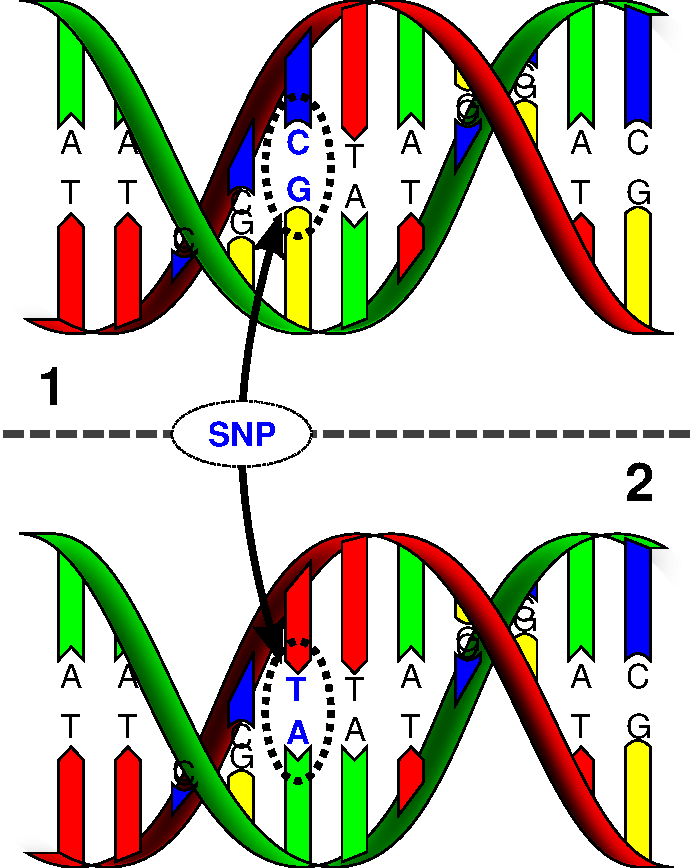
\includegraphics[width=0.4\textwidth]{bilder/DNA_SNP}
	\end{center}
	\caption[Visualisierung eines SNP. (aus \protect\url{http://commons.wikimedia.org/wiki/File:Dna-SNP.svg})]{Visualisierung eines SNP. (aus \protect\url{http://commons.wikimedia.org/wiki/File:Dna-SNP.svg})}
	\label{fig:bio:muta:snp}
\end{figure}
Im Mai 2014 waren in der \textit{dnSNP}, einer Datenbank des amerikanischen \textit{National Center for Biotechnologie Information} \citet{NCBI2014} 62.387.983 SNPs verzeichnet\footnote{Im Jahr 1999 waren erst 7000 SNPs öffentlich bekannt \citep{Brookes1999}}. Auf Grund dieser Vielzahl sind diese Varianten Ursache für die Unterschiede zwischen verschiedenen Menschen, bei beispielsweise Haut- und Haarfarbe oder Körpergröße und -form. Auch sind sie für die Empfänglichkeit von Krankheiten verantwortlich.

Da die Veränderungsrate bei $10^{-8}$ Änderungen pro Nucelotid und Generation liegt, sind einzelne Allele sind sehr stabil \citep{Brookes1999} \citep{Li1996}. 

Um die DNA eines Organismus überhaupt erstmal untersuchen zu können, muss diese sequenziert werden. Die Grundideen und verschiedene Arten der Sequenzierung werden im folgenden Abschnitt beschrieben.
\section{Sequenzierung}
\label{sec:bio:seq}
\marginpar{Jan}

Die Sequenzierung bezeichnet eine Methode zur Bestimmung der Nukleotid-Abfolge der untersuchten DNA. Seit 1977 wurden dabei verschiedene Methoden entwickelt, welche sich in Funktionsweise und Leistung deutlich unterscheiden. Die ersten entwickelten Verfahren waren dabei die chemische Methode von \textsc{Maxam} und \textsc{Gilbert} und die deutlich überlegendere Kettenabbruchmethode von \citet{Sanger1977}, welche nachfolgend vorgestellt wird. Alle weiteren Methoden, die zeitlich später entwickelt wurden, werden auch als \textbf{Next-Generation Sequencing} bezeichnet, von denen einige weitere im Verlauf dieses Kapitels vorgestellt werden.
\subsection{Kettenabbruchmethode}
\label{sec:bio:seq:kette}
\marginpar{Jan}

Die Kettenabruchmethode (auch als \textit{Dideoxy-Methode} bezeichnet) sequenziert eine eingebrachte DNA mittels Synthese durch eine Polymerase \citep{Jansohn2011}. 

Zur Vorbereitung muss die zu untersuchende DNA in hoher Stückzahl verfügbar sein. Die Klonierung erfolgt beispielsweise mit der in Abschnitt \ref{sec:bio:zell:pcr} vorgestellten Technik \textit{PCR}. Die Polymerase verlängert nun einen eingebrachten Primer, dessen Sequenz bekannt ist, so dass ein Komplement entsteht. In jedem Zyklus wird ein markiertes Nukleotid, ein sogenanntes \textit{Didesoxyribonukleosid-Triphosphat} (ddNTP), eingebracht. Diese besitzen am 3' Ende keine Hydroxygruppe. Da sich dort normalerweise die Verbindung zum nächsten Nukleotid befindet, kommt es beim Einbau eines ddNTP zum Abbruch der Kette und die Synthese terminiert.
\begin{figure}[htb]
	\begin{center}
		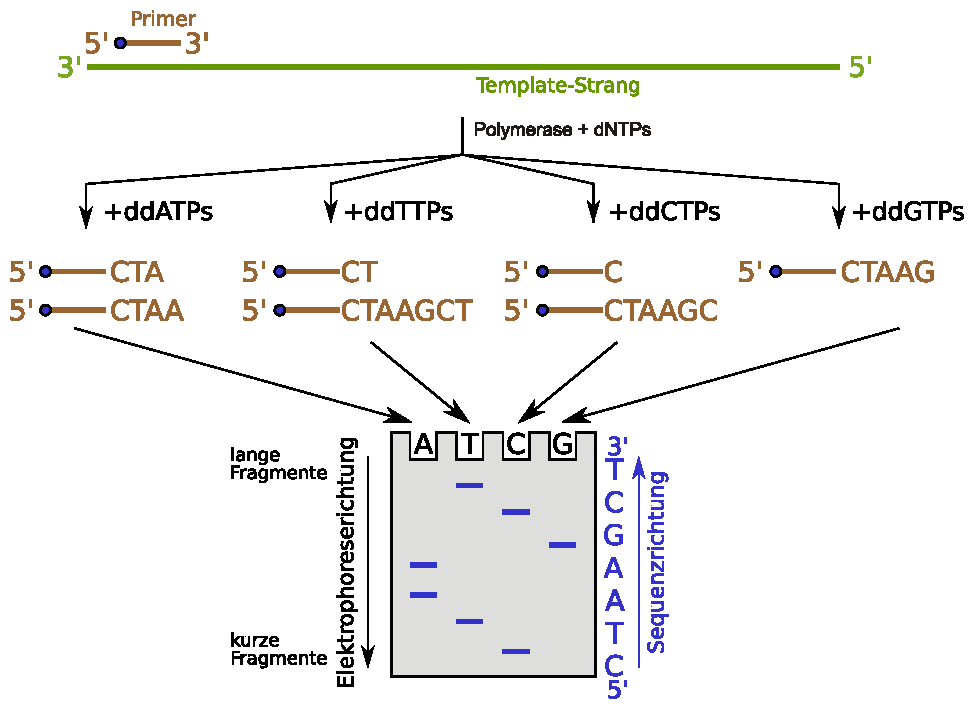
\includegraphics[width=0.6\textwidth]{bilder/Sequenzierung_Kettenabbruch}
	\end{center}
	\caption[Visualisierung der Kettenabbruchmethode nach Sanger. (aus \protect\url{http://commons.wikimedia.org/wiki/File:Didesoxy-Methode.svg})]{Visualisierung der Kettenabbruchmethode nach Sanger. (aus \protect\url{http://commons.wikimedia.org/wiki/File:Didesoxy-Methode.svg})}
	\label{fig:bio:seq:kette}
\end{figure}
Dadurch entsteht eine Vielzahl von DNA-Fragmenten mit unterschiedlichen Längen. Das Ablesen der Kodierung erfolgt in einer \textit{Elektrophorese}. Kurze Fragmente wandern, wie in Abbildung \ref{fig:bio:seq:kette} illustriert, am weitesten. Durch die Markierungen des jeweils letzten Nukleotids jedes Fragments lässt sich der genetische Code schrittweise erweitern. 

In der Vergangenheit nutzte man eine radioaktive Markierung der Nukleotide. Um das Gefahrenrisiko zu senken, wurden verschiedene fluoreszierende Markierungen verwendet %was sich vorteilhaft auf die Nutzung auswirkte?. 
Die entstehenden Reads besitzen eine Länge von bis zu 1000 Basenpaaren, dessen Sequenzierung Kosten in Höhe von $\$0{,}50$ pro Tauschend Basenpaaren verursachten. Auch wurde eine hohe Genauigkeit von bis zu $99{,}9 \%$ erzielt \citep{Shendure2008}. Leider ist die Kettenabbruchmethode aufwendig und kostet viel Zeit. Daher wurden neue Sequenziertechniken entwickelt, welche nachfolgend vorgestellt werden.
\newline
\subsection{Cyclic reversible termination (CRT)}
\label{sec:bio:seq:crt}
\marginpar{Jan}

Die Sequenziermethode \emph{CRT} (Cyclic reversible termination) nutzt ebenfalls einen Abbruch der Kette zur Nukleotidbestimmung aus. Im Gegensatz zur Methode von Sanger ist dieser Abbruch aber reversibel und benötigt keine Klonierung in hoher Anzahl. In jedem Zyklus wird versucht, genau ein farblich markiertes Nukleotid an den komplementären Strang der zu untersuchenden DNA zu binden. Der angesprochene \textit{reversible Terminator} unterbricht die Bindung von weiteren Molekülen. Nachdem die Fluoreszenz gemessen wurde und damit das gebundene Nukleotid identifiziert wurde, muss der fluoreszierende Terminator von der DNA gespalten werden, bevor der nächste Zyklus beginnt.

Wahlmöglichkeiten gibt es bei der Art der Markierung. Die erste Möglichkeit besteht darin, gleichzeitig alle vier verschiedenen Nukleotide hinzuzufügen, wobei jedes eine andere Fluorophore zur Identifikation erhält. Die andere Möglichkeit sieht für jedes Molekül denselben Farbstoff vor. In jedem Zyklus muss dabei darauf geachtet werden, dass ein anderes dNTP hinzugefügt wird, um die korrekte Sequenz ermitteln zu können. 

Die entstehenden Reads hatten bei Verwendung der ersten Maschinen dieser Plattform eine Länge von ca. 30 Basenpaaren, die neuen Modelle erreichen Längen von über 100 Basenpaaren \citep{Metzker2010}.
\subsection{Sequenzierung durch Hybridisierung}
\marginpar{Jan}

Diese Art der Sequenzierung nutzt den Umstand aus, dass sich passende DNA-Einzelstränge unter geeigneten Bedingungen zu einem komplementären Doppelstrang zusammensetzen. Zur Vorbereitung wird eine Vielzahl von DNA-Sonden, sogenannten \textit{Oligonukleotiden} mit einer bekannten Folge von 4 - 8 Nukleotiden, an einer festen Oberfläche befestigt \citep{Gresham2008}. Möglich ist auch die Nutzung von industriell gefertigten DNA-Chips. Die zu untersuchenden DNA-Abschnitte werden farblich markiert und hinzugefügt. Durch Untersuchung der Markierungen an den Positionen der Oligonukleotide kann entschieden werden, ob eine Bindung stattfand. Fällt das Ergebnis positiv aus, kann die Sequenz dieses Reads durch Komplementierung der Basenabfolge des jeweiligen Oligonukleotids bestimmt werden.
\subsection{Pyrosequezierung}
\label{sec:bio:seq:pyro}
\marginpar{Jan}

Das Grundvorgehen der Pyrosequenzierung ist die Beobachtung einer DNA-Replikation. Zur Vorbereitung werden die folgenden vier Enzyme zugegeben: DNA-Polymerase, ATP-Sulfurylase, Luciferase, Apyrase \citep{Ahmadian2006}. \\
Die eigentliche Sequenzierung läuft nun zyklenweise ab. Die Polymerase sucht ein freies Nukelotid, welches an den komplementären DNA-Strang andocken kann. Iterativ werden jeweils die Desoxyribonukleosidtriphosphate dATP, dCTP, dGTP, dTTP hinzugefügt. Kann ein Nukleotid andocken, wird durch die Polymerase \textit{Pyrophosphat} freigesetzt, welches dann durch ein weiteres Enzym, der ATP-Sulfurylase, zu \textit{Adenosintriphosphat (ATP)} umgewandelt wird. Die Luciferase, welche ursprünglich aus Glühwürmchen extrahiert wurde, katalysiert das ATP zu einem Lichtblitz \citep{Ahmadian2006}. Somit ist klar: Tritt ein Lichtblitz auf, konnte die Polymerase das aktuelle Nukleotid binden und bildet ein weiteres Glied der Sequenz. 
\begin{figure}[H]
	\begin{center}
		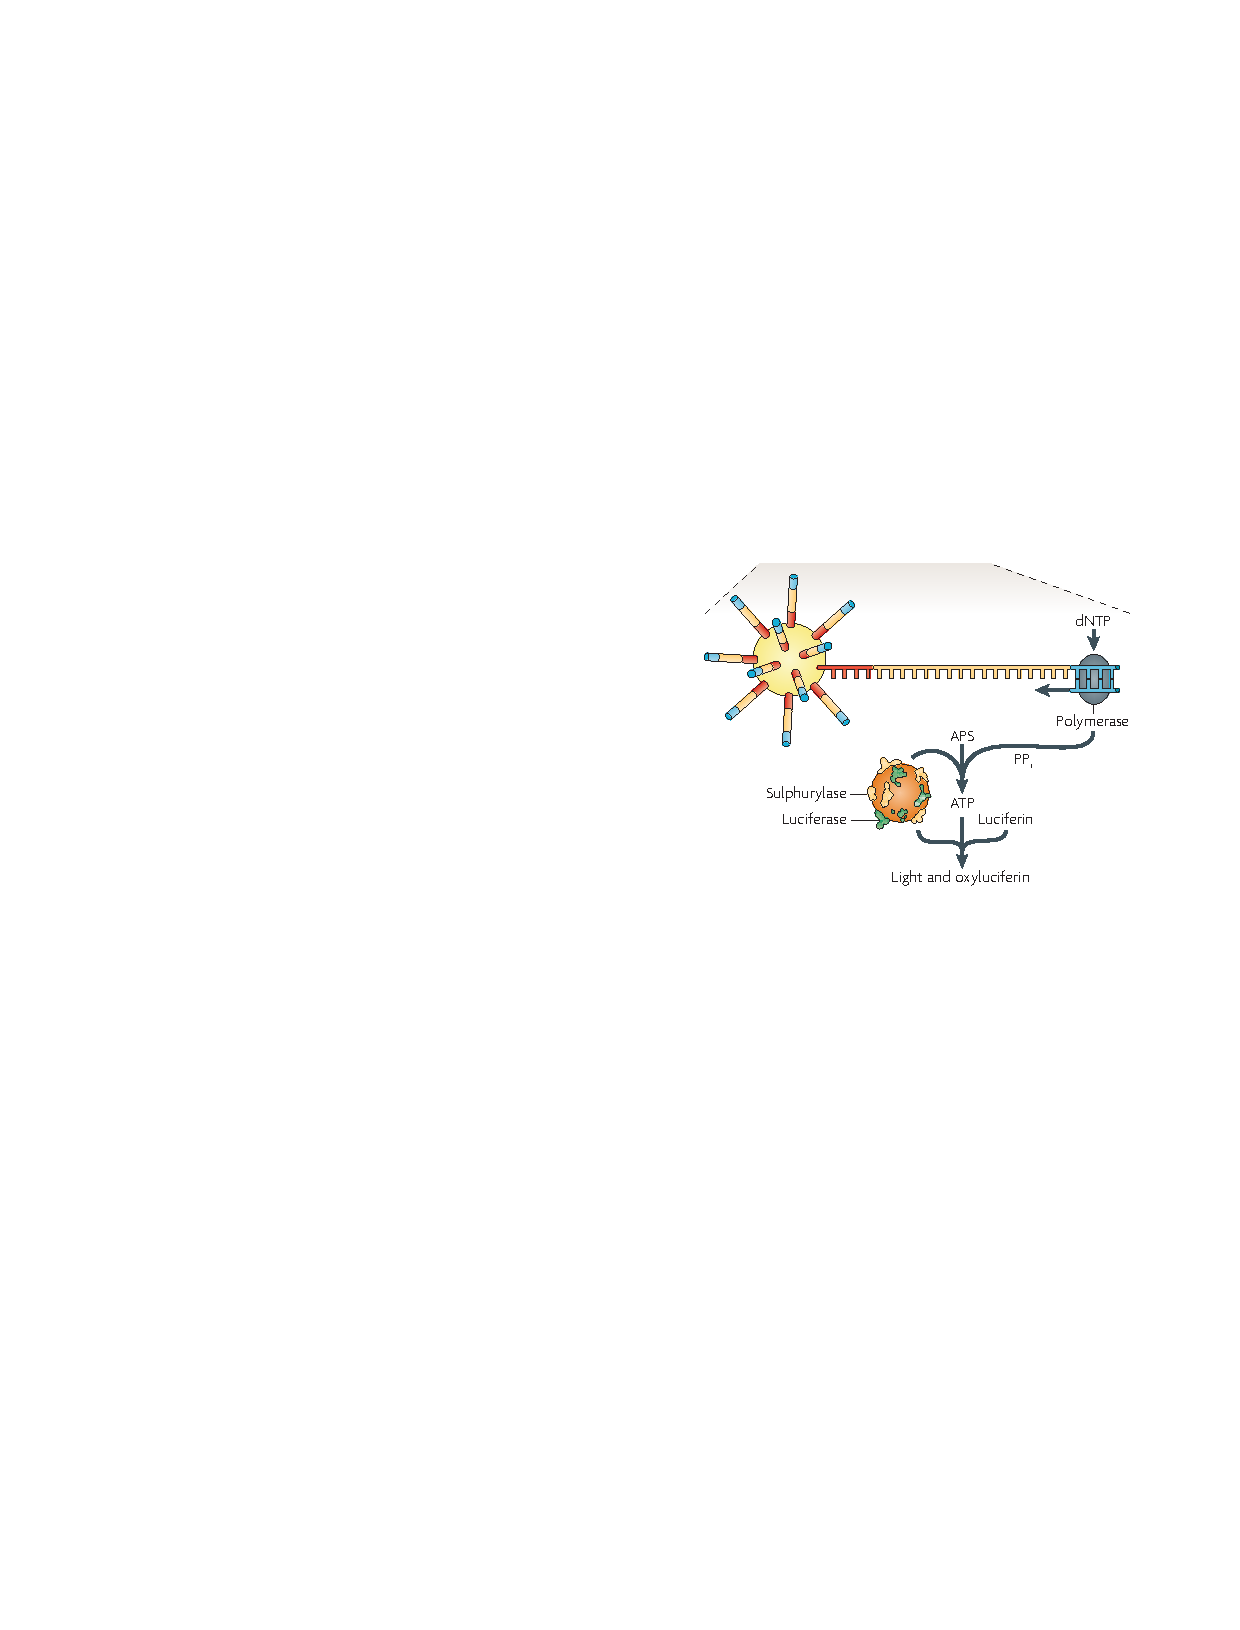
\includegraphics[width=0.6\textwidth]{bilder/Sequenzierung_Pyro_Schema}
	\end{center}
	\caption{Darstellung der Pyrosequenzierung (aus \citet{Metzker2010})}
	\label{fig:bio:seq:pyro:schema}
\end{figure}
Nach mehreren Zyklen und der Zugabe der verschiedenen dNTPs lässt sich der gesamte Read konstruieren. Die gesamte Beobachtung der Sequenzierung muss dabei in Echtzeit erfolgen, damit die Lichtblitze den richtigen dNTPs zugeordnet werden können \citep{Shendure2008}. Außerdem ist wichtig, dass auch die Intensität des Lichtblitzes gemessen wird, welche proportional zur Anzahl der eingebauten Nukleotide steigt. Für die Sequenz bedeutet dies, falls ein Lichtblitz mit doppelter Intensität auftritt, kommt das entsprechende Nukleotid zweimal vor. 
\begin{figure}[H]
	\begin{center}
		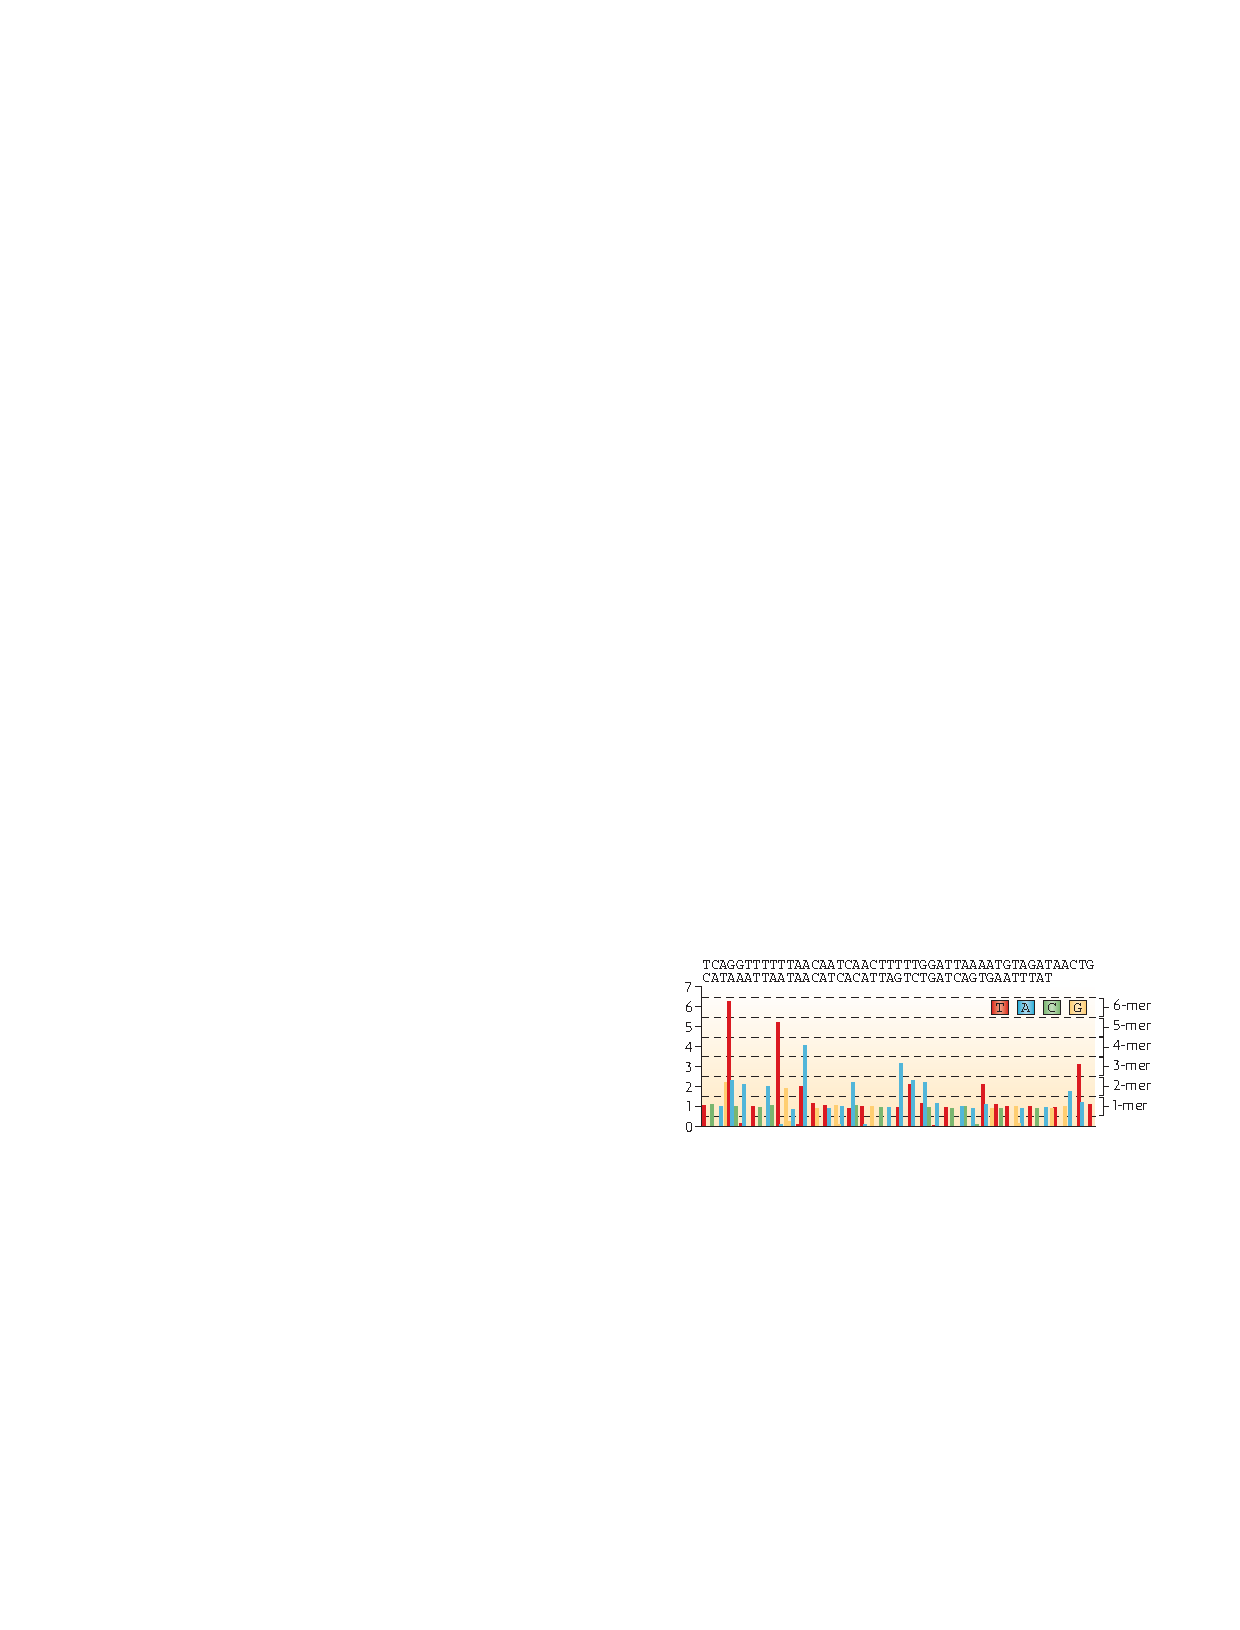
\includegraphics[width=0.8\textwidth]{bilder/Sequenzierung_Pyro_Diagramm}
	\end{center}
	\caption{Intensität der Lichtblitze (aus \citet{Metzker2010})}
	\label{fig:bio:seq:pyro:diagram}
\end{figure}
Ein großer Vorteil der Pyrosequenzierung ist die hochparallele Generierung von hunderttausenden Reads mit einer Länge von bis zu 400 Basenpaaren. Auch ist es möglich, dass verschiedene Proben gleichzeitig analysiert werden können, was sich kostensenkend auswirkt \citep{Siqueira2012}. Durch die langen Reads ist eine zuverlässige Erkennung von SNPs möglich, jedoch ist die Fehlerrate bei der Erkennung von Indels hoch, da \textit{Homopolymere}, also Wiederholungsfolgen derselben Base, nur anhand der verschiedenen Intensität der Lichtblitze erkannt werden können \citep{Shendure2008}.
\subsection{Echtzeit-Sequenzierung}
\label{sec:bio:seq:realtime}
\marginpar{Jan}

Bei der Echtzeit-Sequenzierung kann die ermittelte DNA-Sequenz direkt durch Beobachtung der Polymerase abgelesen werden. Im Gegensatz zur Pyrosequenzierung, welche ebenfalls in Echtzeit beobachtet werden muss, muss bei diesem Ansatz die DNA-Synthese nicht gestoppt werden. Einzelne Polymerasen werden an der Oberfläche eines Detektors angebracht, der Nukleotide erkennen kann, die um ein fluoreszierendes Phosphat erweitert wurden\citep{Eid2009}. Diese werden in hoher Anzahl hinzugegeben. In jedem Zyklus wird versucht, eines der Nukleotide einzubinden. Ist der Versuch erfolgreich, löst sich das farblich markierte Pyrophosphat und löst einen messbaren Puls aus. Der Detektor misst diesen und setzt daraus die Sequenz zusammen.
\begin{figure}[H]
	\begin{center}
		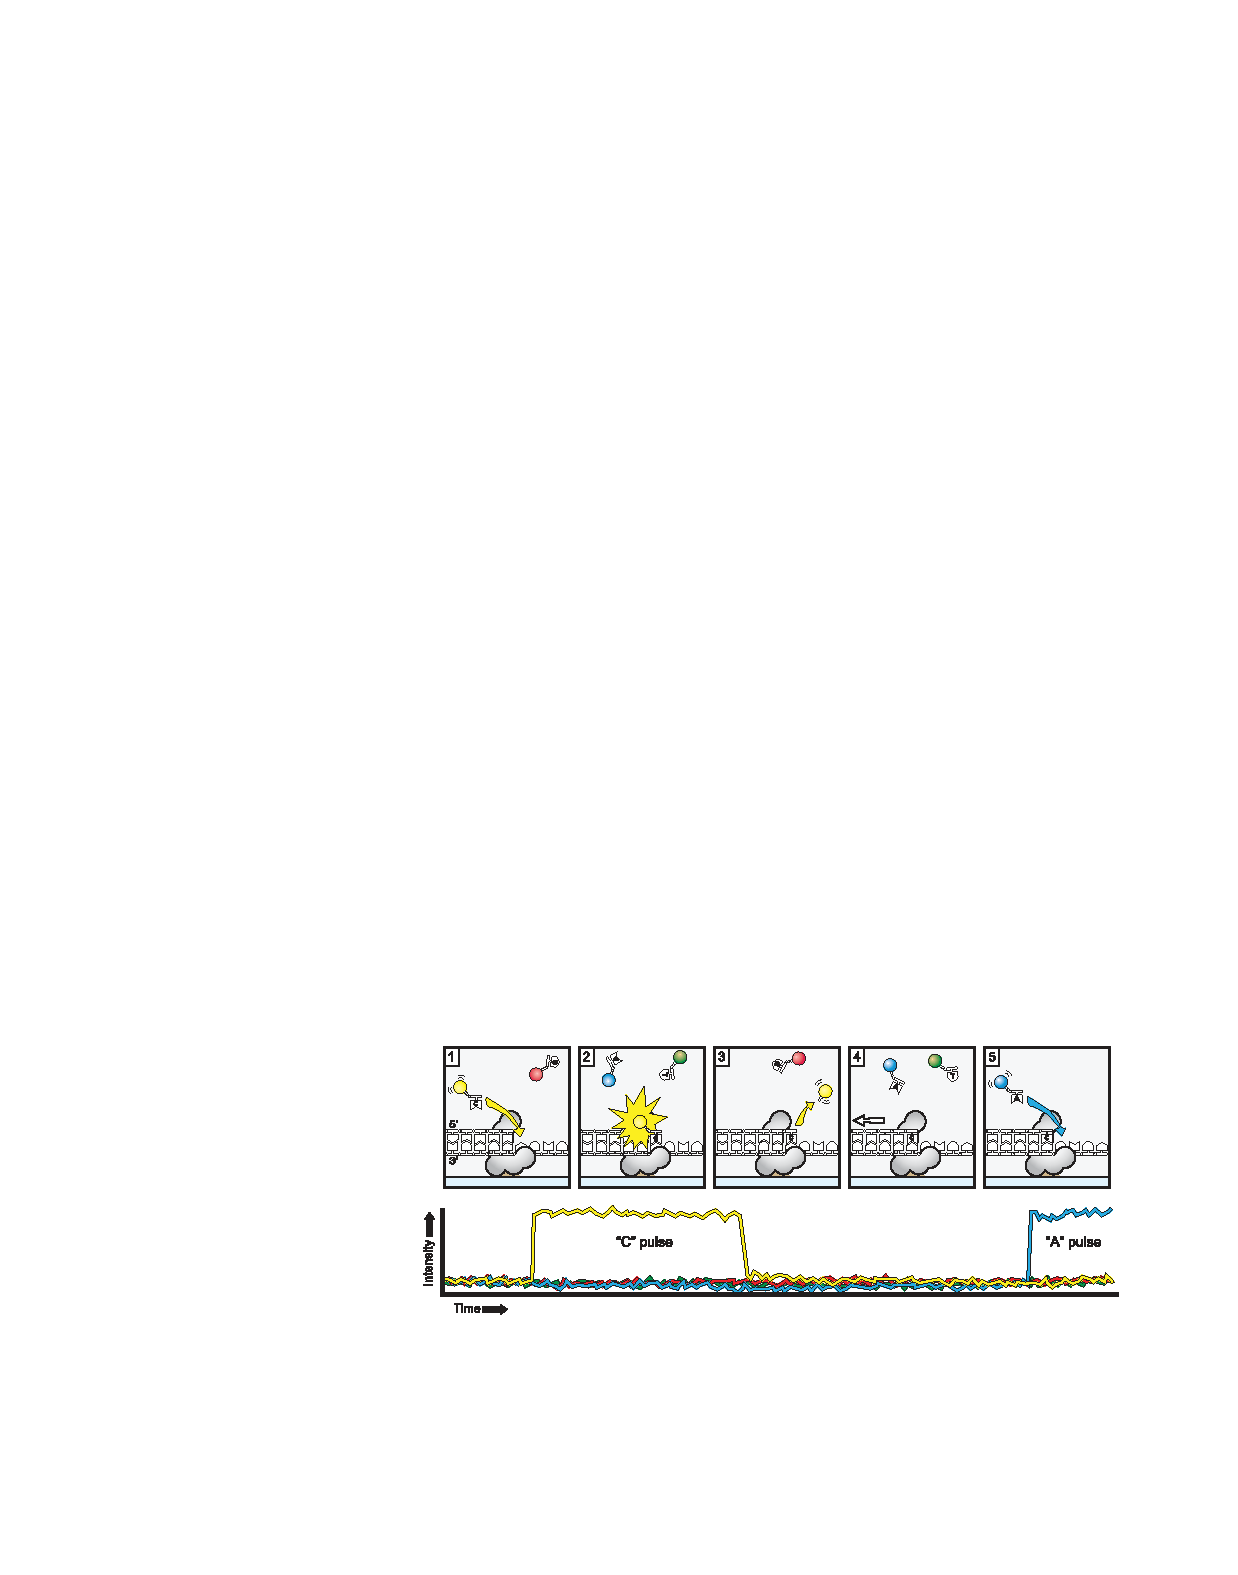
\includegraphics[width=\textwidth]{bilder/Sequenzierung_Realtime}
	\end{center}
	\caption{Darstellung der Echtzeitsequenzierung (aus \citet{Eid2009})}
	\label{fig:bio:seq:realtime}
\end{figure}
	Vorteilhaft wirken sich hohe Readlängen von bis zu 1000 Basenpaaren und die hohe Geschwindigkeit der Sequenzierung aus, welche nur von der Synthesegeschwindigkeit\footnote{Diese Geschwindigkeiten liegen zwischen $0.7$ und $1.5$ Basen pro Sekunde \citep{Eid2009}.} der verwendeten Polymerase abhängig ist \citep{Metzker2010}. Die Genauigkeit eines einzelnen Sequenzierungsdurchgangs ist relativ ungenau ($\sim 83\%$). Durch mehrfache Wiederholung der Sequenzierung desselben Reads lässt sich diese Genauigkeit auf über $99\%$ erhöhen \citep{Eid2009}.
